%\documentclass[handout,xcolor=pdftex,dvipsnames,table,mathserif]{beamer}
\documentclass[xcolor=pdftex,dvipsnames,table]{beamer}
\usepackage{subfigure}
\usepackage{amsbsy}
\usepackage{tikz}
\usetikzlibrary{arrows}
\usepackage{amsmath,graphicx,dsfont,color}
\usepackage{amsfonts}
\usepackage{amssymb}
\usepackage{array}

\bibliographystyle{apalike}

\setbeamertemplate{bibliography item}{\insertbiblabel}
\setbeamertemplate{bibliography entry title}{}
\setbeamertemplate{bibliography entry location}{}
\setbeamertemplate{bibliography entry note}{}

%Definitiona

\newcommand{\x}{\mathbf{x}}
\newcommand{\X}{\mathbf{X}}
\newcommand{\W}{\mathbf{W}} %Weight
\newcommand{\bais}{\mathbf{b}}%Bais
\newcommand{\act}{\texttt{g}}%Activation
\newcommand{\loss}{L}
\newcommand{\pdata}{\hat{p}_{\texttt{data}}}
\newcommand{\nsize}{n}
\newcommand{\param}{\boldsymbol{\theta}}
\newcommand{\featmap}{\boldsymbol{\phi}}
\newcommand{\EV}{\mathbb{E}}









\title{Deep Learning for Image Analysis - \\
	   Object detection}
\author{Thomas Walter, PhD}
\date{Centre for Computational Biology (CBIO) \\
	  MINES Paris-Tech, PSL Research University \\
	  Institut Curie, PSL Research University \\
	  INSERM U900}


%To include LOGO?
%\logo{\includegraphics[width=.1\columnwidth]{MinesLogo}}
\useinnertheme{rounded}
\usecolortheme{rose}

\usepackage[absolute,overlay]{textpos}

\usepackage{xcolor}
\definecolor{lightblue}{RGB}{0,200,255}


\setbeamertemplate{footline}[frame number]{}
\setbeamertemplate{navigation symbols}{}
\setbeamertemplate{section in toc}[square]
\setbeamertemplate{items}[square]

%% For image credits on image bottom right
\usepackage[absolute,overlay]{textpos}
\setbeamercolor{framesource}{fg=gray}
\setbeamerfont{framesource}{size=\tiny}
\newcommand{\source}[1]{\begin{textblock*}{4cm}(8.7cm,8.6cm)
    \begin{beamercolorbox}[ht=0.5cm,right]{framesource}
      \usebeamerfont{framesource}\usebeamercolor[fg]{framesource} Credits: {#1}
    \end{beamercolorbox}
\end{textblock*}}


\begin{document}

\begin{frame}
\titlepage
\end{frame}

\begin{frame}{Overview}
\tableofcontents
\end{frame}

%%%%%%%%%%%%%%%%%%%%%%%%%%%%%%%%%%%%%%%%%%%%%%%%%%%%%%%%%%%%%%%%%%%%%%%%%
%%%%%%%%%%%%%%%%%%%%%%%%%%%%%%%%%%%%%%%%%%%%%%%%%%%%%%%%%%%%%%%%%%%%%%%%%
\section{Introduction}
\frame{\frametitle{Overview}\tableofcontents[currentsection]}

% \begin{frame}{Definition of Artificial Intelligence and Machine Learning}
% %\begin{definition}
% %	Artificial intelligence (AI) is intelligence demonstrated by machines, in contrast to the natural intelligence displayed by humans and other animals.
% %\end{definition}
% \begin{itemize}
% 	\item The definition of the term \textbf{intelligence} is highly controversial. Usually, one understands by intelligence the capacity of an individual to reason logically, to understand complexity, to learn more or less abstract concepts, to plan and to solve problems in varying conditions.
% 	\item \textbf{Artificial intelligence (AI)} is intelligence demonstrated by machines, in contrast to the natural intelligence displayed by humans and other animals.
% 	\item AI effect: \emph{"AI is whatever hasn't been done yet"}.
% 	\item In 1956, AI became a field of research. AI can be broken down into many subfields: knowledge representation, planning, natural language processing, object manipulation (robotics), machine learning, $\ldots$
% 	\item \textbf{Machine Learning} is concerned with the technology that enables computer programs to improve their performance at a certain task by experience.
% \end{itemize}
% \end{frame}

% \begin{frame}{A short history of artificial intelligence}
% \begin{itemize}
% 	\item The dream to create machines that can think and act has been present in literature and mythology since antiquity (e.g. the myth of \emph{"Talos"} or \emph{"Rossum's Universal Robots"} by Karel \v{C}apek, 1920).
% 	\item AI as a scientific discipline took its beginning with the publication of Alan Turing in 1950 (Turing test). The question \emph{"Can machines think?"} was asked scientifically.
% 	\item Other theoretical bases were developed by Wiener (cybernetics) and Shannon (information theory).
% 	\item The term \emph{"artificial intelligence"} was cornered in 1956, in the famous Dartmouth conference, where AI has been established as a field.
% \end{itemize}
% \end{frame}

% \begin{frame}{A short history of machine learning}
% \begin{figure}[htb]
%   \centering
%   \subfloat{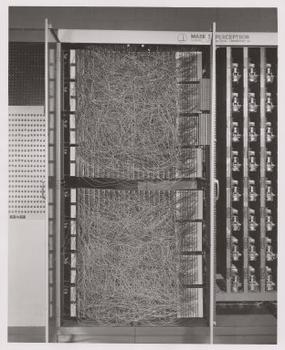
\includegraphics[height=0.23\textheight]{../graphics/Mark_1_perceptron.jpeg}}\hspace{2cm}
%   \subfloat{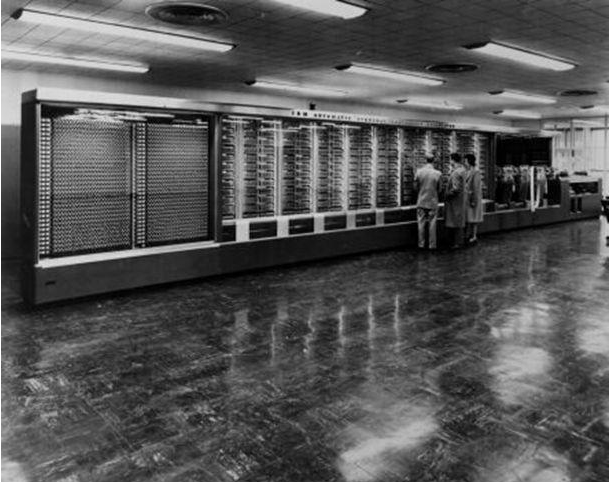
\includegraphics[height=0.23\textheight]{../graphics/perceptron.jpg}}
%   \caption{The Mark I Perceptron}
% \end{figure}
% \vspace{-.5cm}
% \begin{itemize}
% 	\item The theoretical foundations go back to the early 19th century (e.g. Bayesian theory and Least Squares).
% 	\item Even before machines came into play, there was a lot of interest in finding methods to derive rules from data (\emph{data fitting}). These methods are part of what we call Machine Learning today (linear regression, Bayesian theory, Logistic regression, Linear discriminant analysis, Markov chains).
% 	\item In 1958, Rosenblatt published his \emph{Perceptron} (basically a linear classifier), which is seen as the predecessor of Neural Networks.
% \end{itemize}
% \end{frame}
\begin{frame}{Classification, segmentation and detection}
% \begin{figure}[htb]
%   \centering
%   \subfloat{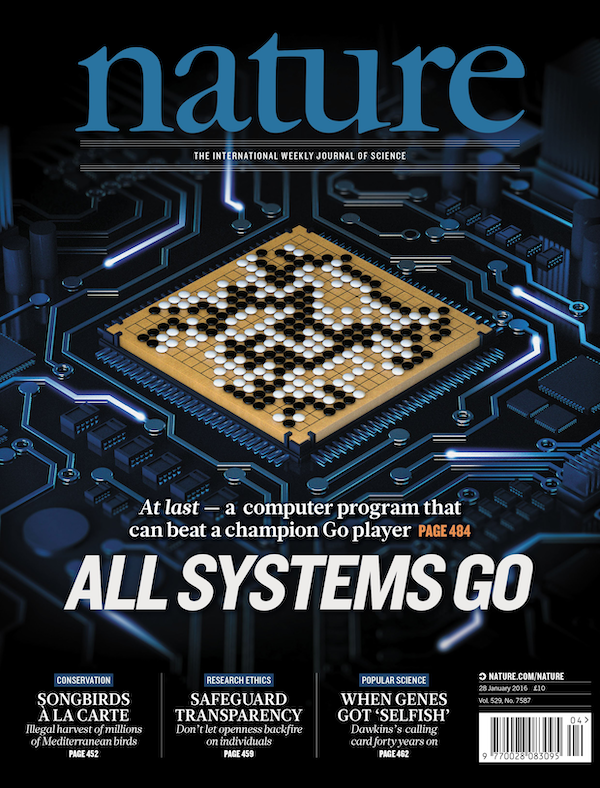
\includegraphics[height=0.6\textheight]{../graphics/NatureGo.png}}\hspace{2cm}
%   \subfloat{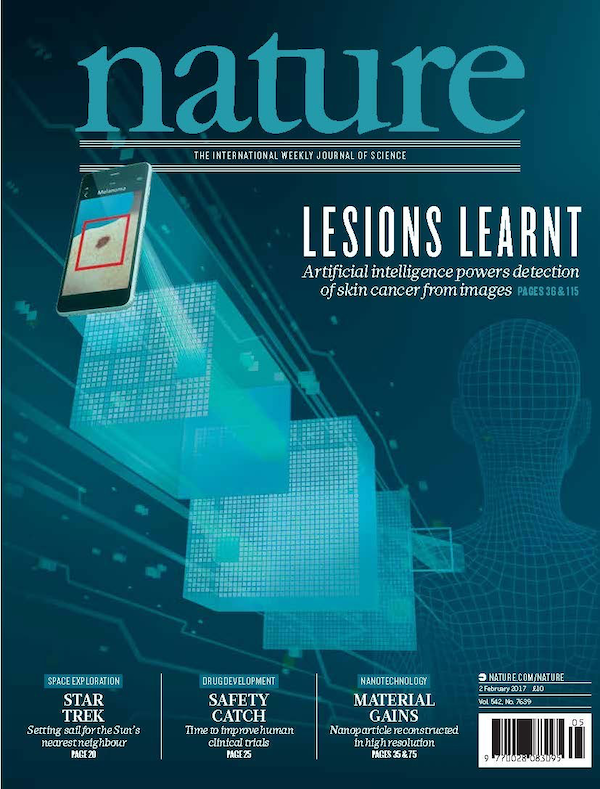
\includegraphics[height=0.6\textheight]{../graphics/NatureSkinLesions.png}}
%   \caption{Two recent success stories of Artificial Intelligence: AI beats the world champion in GO and dermatologists in skin cancer detection.}
% \end{figure}
\begin{itemize}
	\item Image Classification: assign a label to each image. 
	\item Semantic image Segmentation: partition the image, i.e. assign a label to each pixel.   
	\item Object detection: detect instances of semantic objects of certain classes in images \cite{Ren2017, Zhao2019}.
	\item Object detection has thus two components:
	\begin{itemize}
		\item \textit{Object localization:} to determine where objects are located in a given image
		\item \textit{Object classification:} which category each object belongs to
	\end{itemize}
   \item (Multiple) instance Segmentation: combines the objectives of object detection and segmentation.
   % \begin{itemize}
   %    \item Segments individual objects
   %    \item Refines object detection.
   % \end{itemize}
\end{itemize}
%\vspace{-.5cm}
\end{frame}

\section{Localization and classification}
\begin{frame}{Localization and classification}
\begin{figure}[htb]
   \centering
   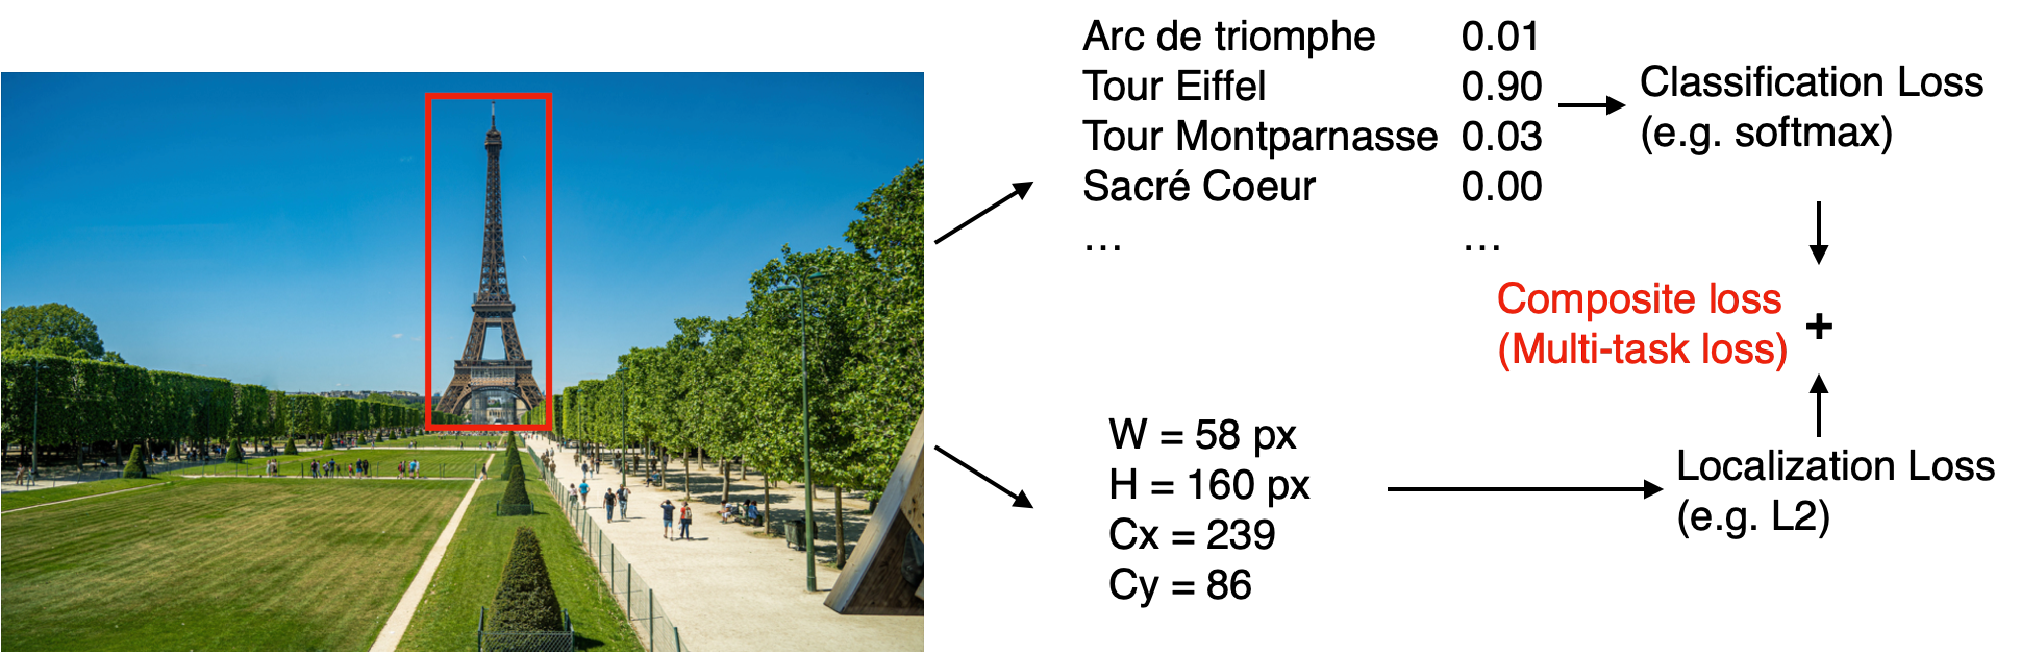
\includegraphics[width=0.95\textwidth]{../graphics/class_and_loc.pdf}
   \caption{Object detection: classification and localization}
\end{figure}
\begin{itemize}
\item Simplified example: one centered object of interest
\item Tasks: 
\begin{itemize}
   \item \textbf{Classification: } classification of the object's content.
   \item \textbf{Localization: } regression on the position / extension.
\end{itemize}
\end{itemize}
\end{frame}

\section{Localization and classification}
\begin{frame}{Localization and classification}
\begin{figure}[htb]
   \centering
   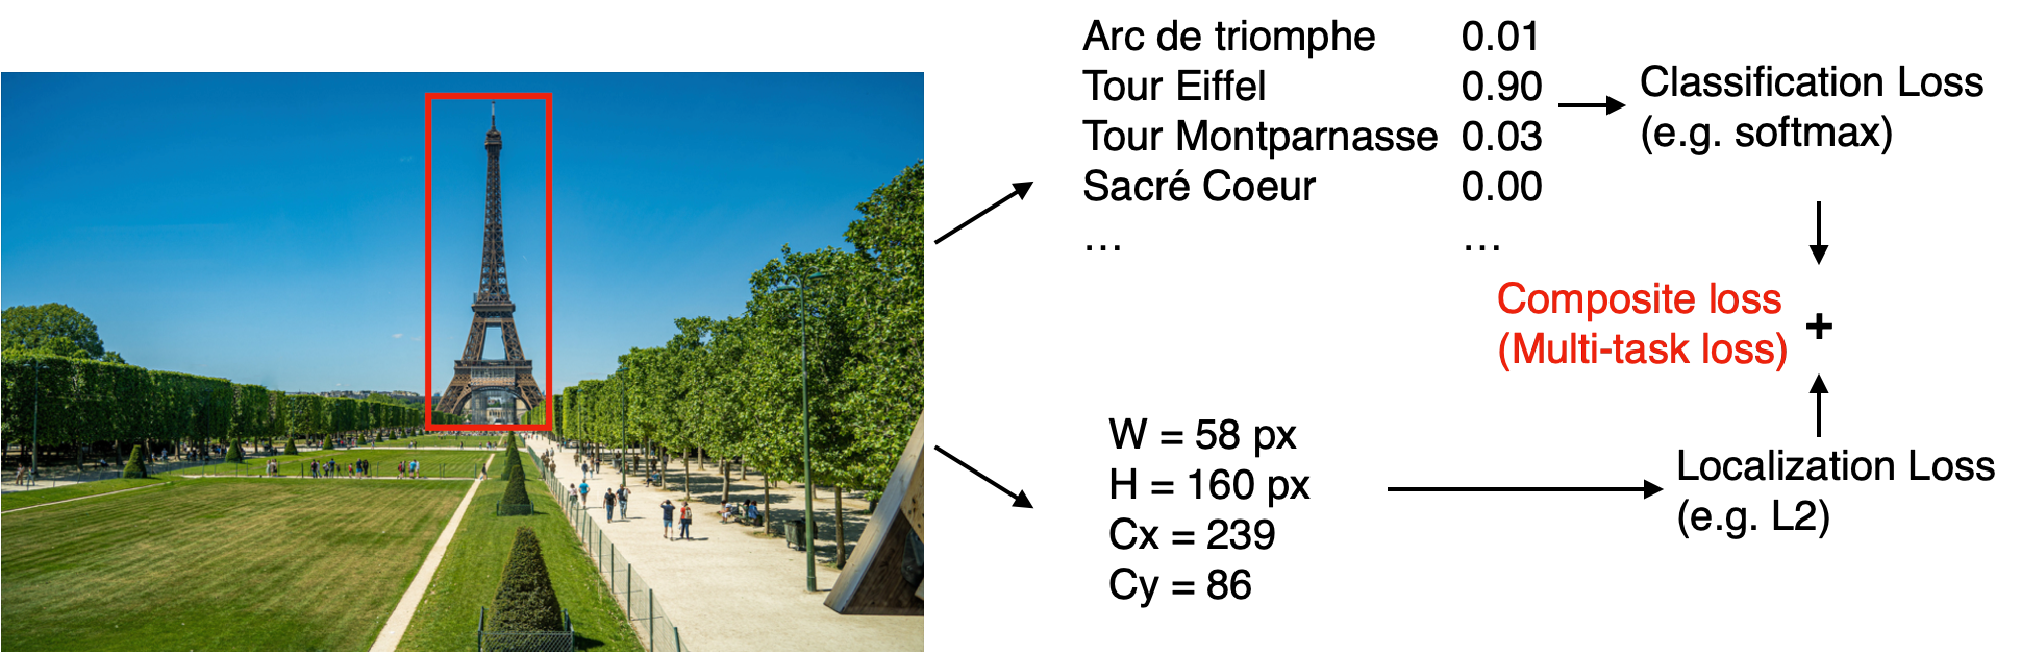
\includegraphics[width=0.95\textwidth]{../graphics/class_and_loc.pdf}
   \caption{Object detection: classification and localization}
\end{figure}
\begin{itemize}
   \item Two tasks from the same image, with two contributions to the loss.
   \item Classification loss (e.g. softmax)
   \item Localization loss (e.g. regression loss on position and extension of a bounding box)
\end{itemize}
\end{frame}

\begin{frame}{Object detection: example}
\begin{figure}[htb]
   \centering
   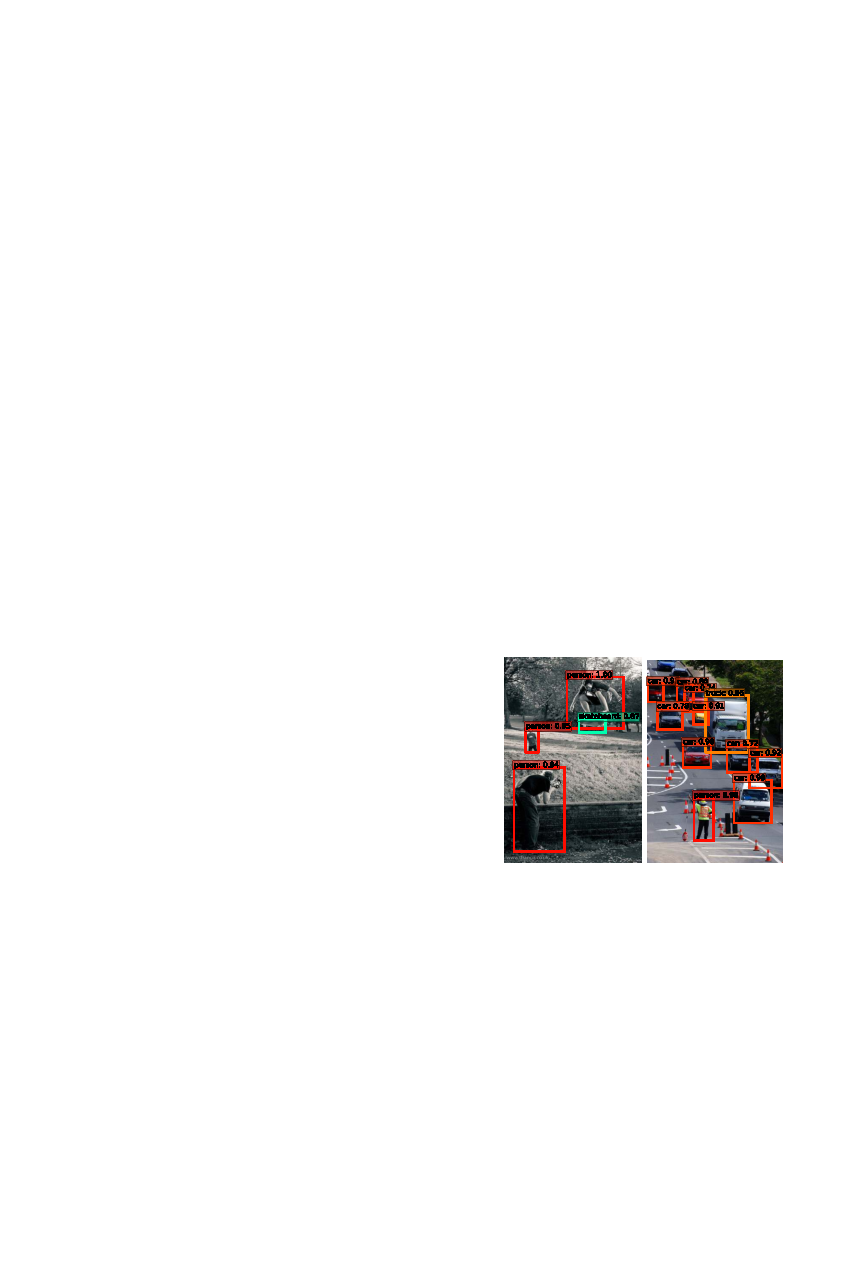
\includegraphics[width=0.95\textwidth]{../graphics/Detection_example1.pdf}
   \caption{Object detection in action. Image taken from \cite{Liu2016}}
\end{figure}
\end{frame}

\begin{frame}{Object detection: example}
\begin{figure}[htb]
   \centering
   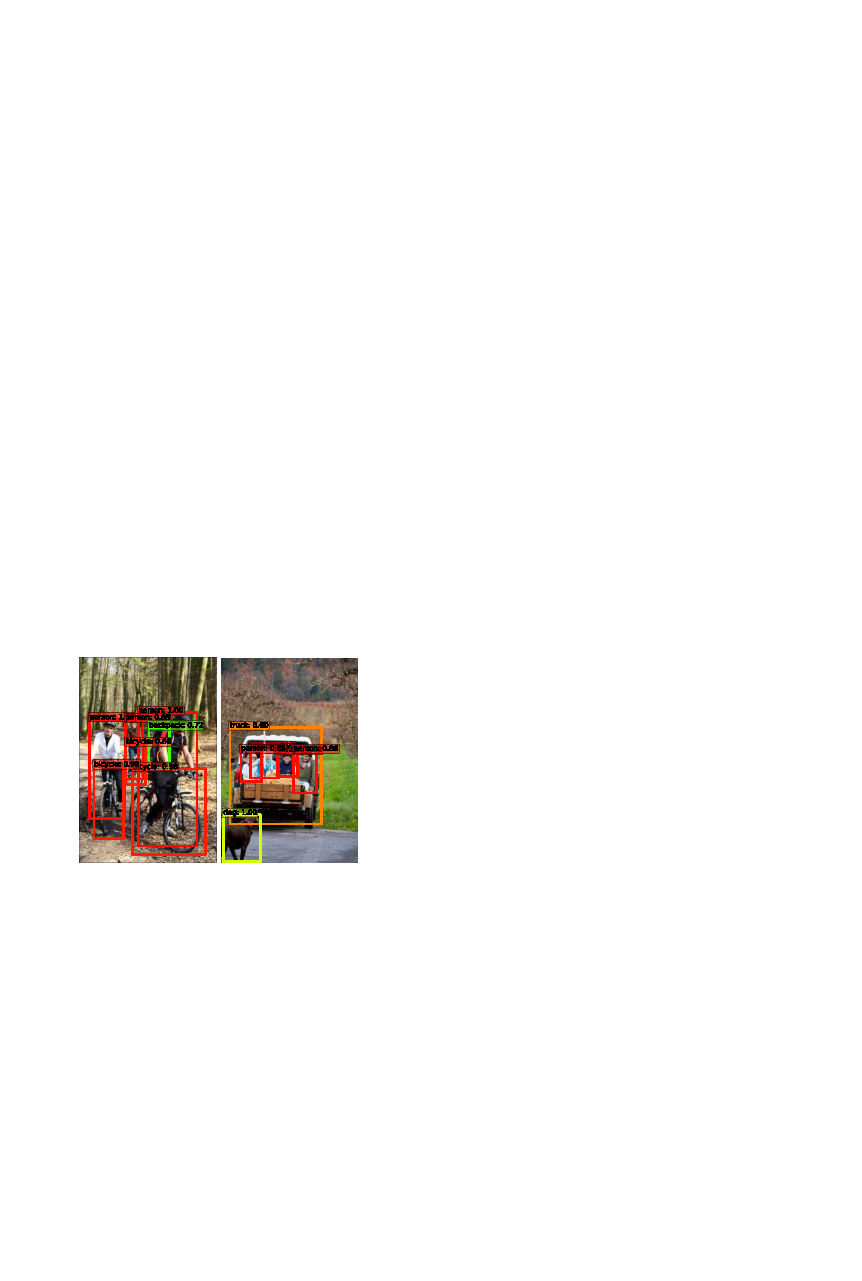
\includegraphics[width=0.95\textwidth]{../graphics/Detection_example2.pdf}
   \caption{Object detection in action. Image taken from \cite{Liu2016}}
\end{figure}
\end{frame}

\begin{frame}{Object detection: example}
\begin{figure}[htb]
   \centering
   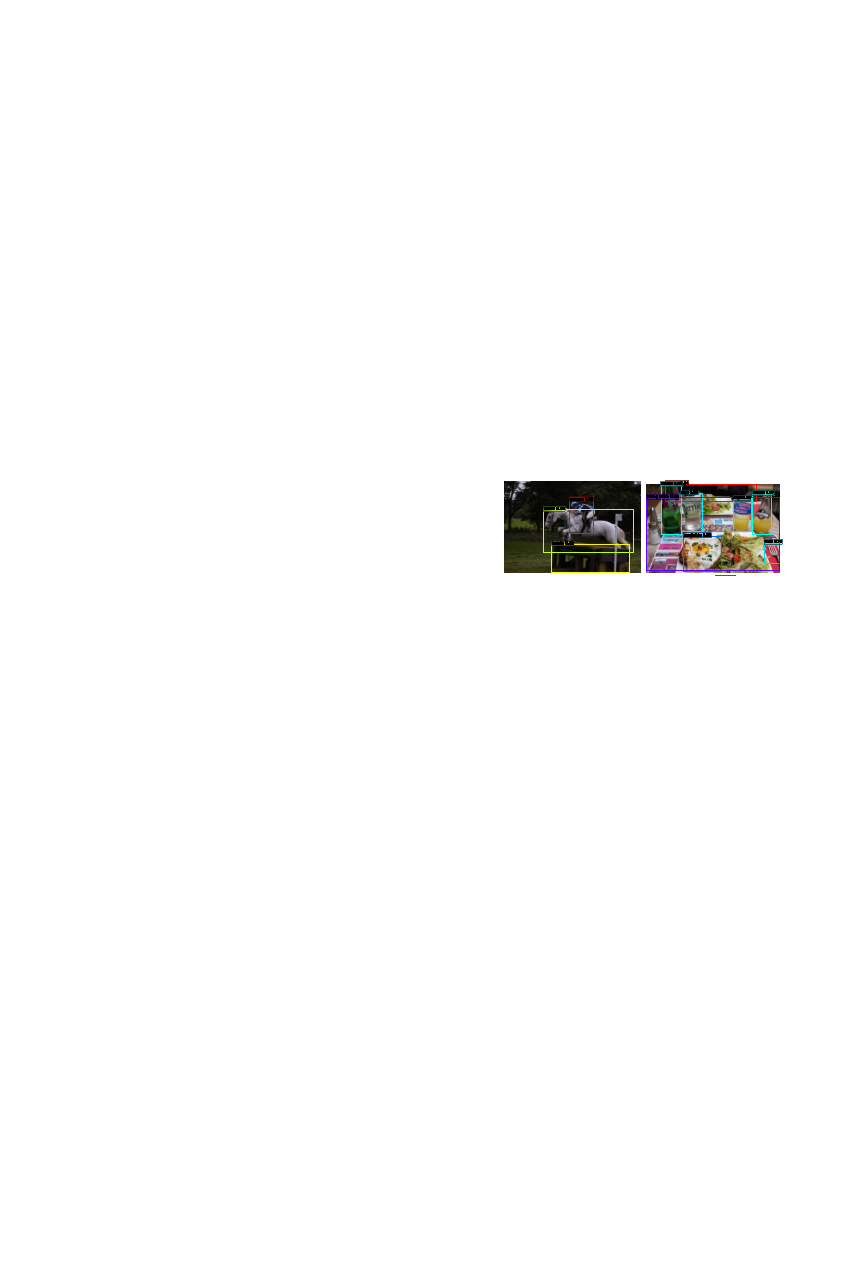
\includegraphics[width=\textwidth]{../graphics/Detection_example3.pdf}
   \caption{Object detection in action. Image taken from \cite{Liu2016}}
\end{figure}
\end{frame}


% \begin{frame}{Difficulties in object detection}
% \begin{itemize}
% \item Orientation: an object can appear under any variation in the image. 
% \end{itemize}
% \end{frame}

\section{Architectures for object detection}
\begin{frame}{Early approaches: the sliding window approach}
\begin{figure}[htb]
   \centering
   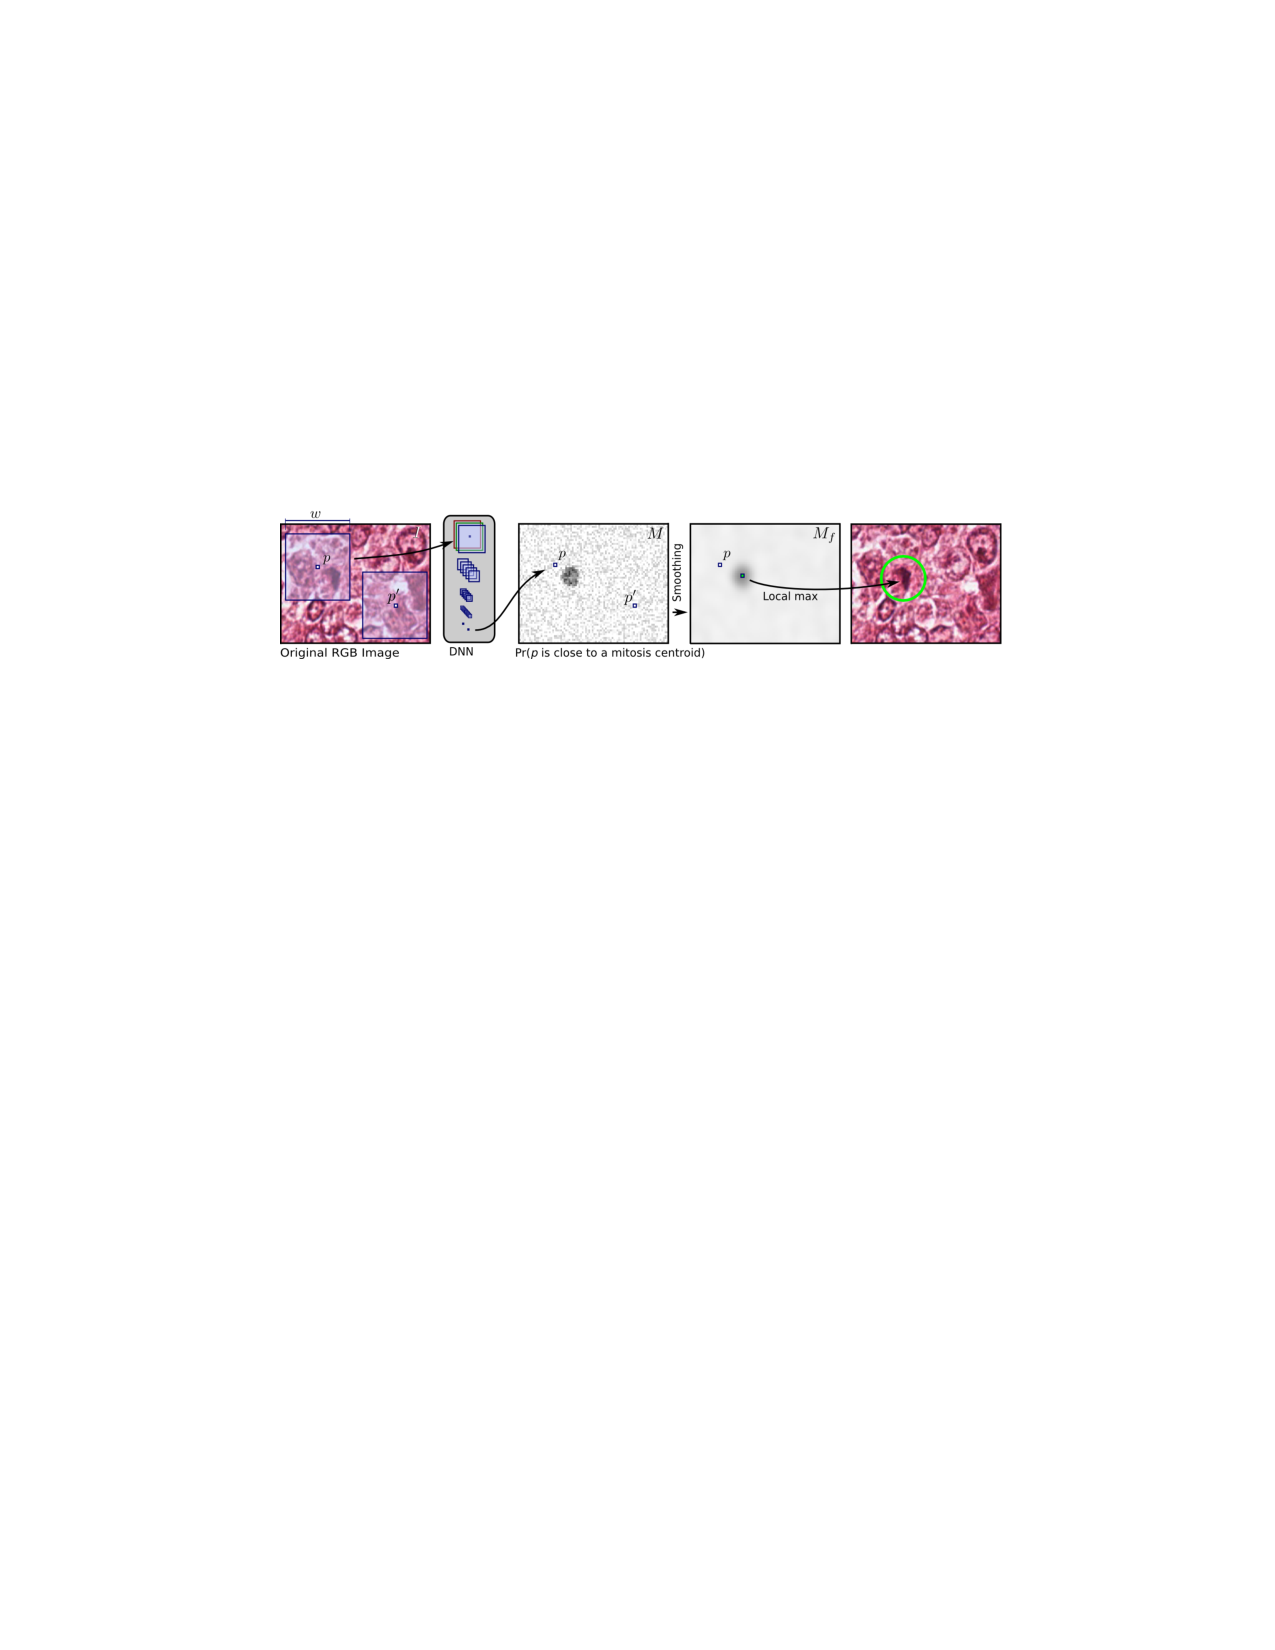
\includegraphics[width=0.8\textwidth]{../graphics/mitosis_detection.pdf}
   \caption{Mitosis detection in stained tissue sections \cite{Ciresan2013}.}
\end{figure}

\begin{itemize}
\item Approach was the winner of a mitosis detection challenge \cite{Ciresan2013}. 
\item Fixed size sliding window approach: each crop is presented to a CNN.
\item The posterior probability is stored as an image value.
\item Local maxima of this probability map indicate the presence of an object.
\item Special case of object detection: the size of the objects was known before.
\end{itemize}
\end{frame}

\begin{frame}{A milestone in object detection: R-CNN}
\begin{figure}[htb]
   \centering
   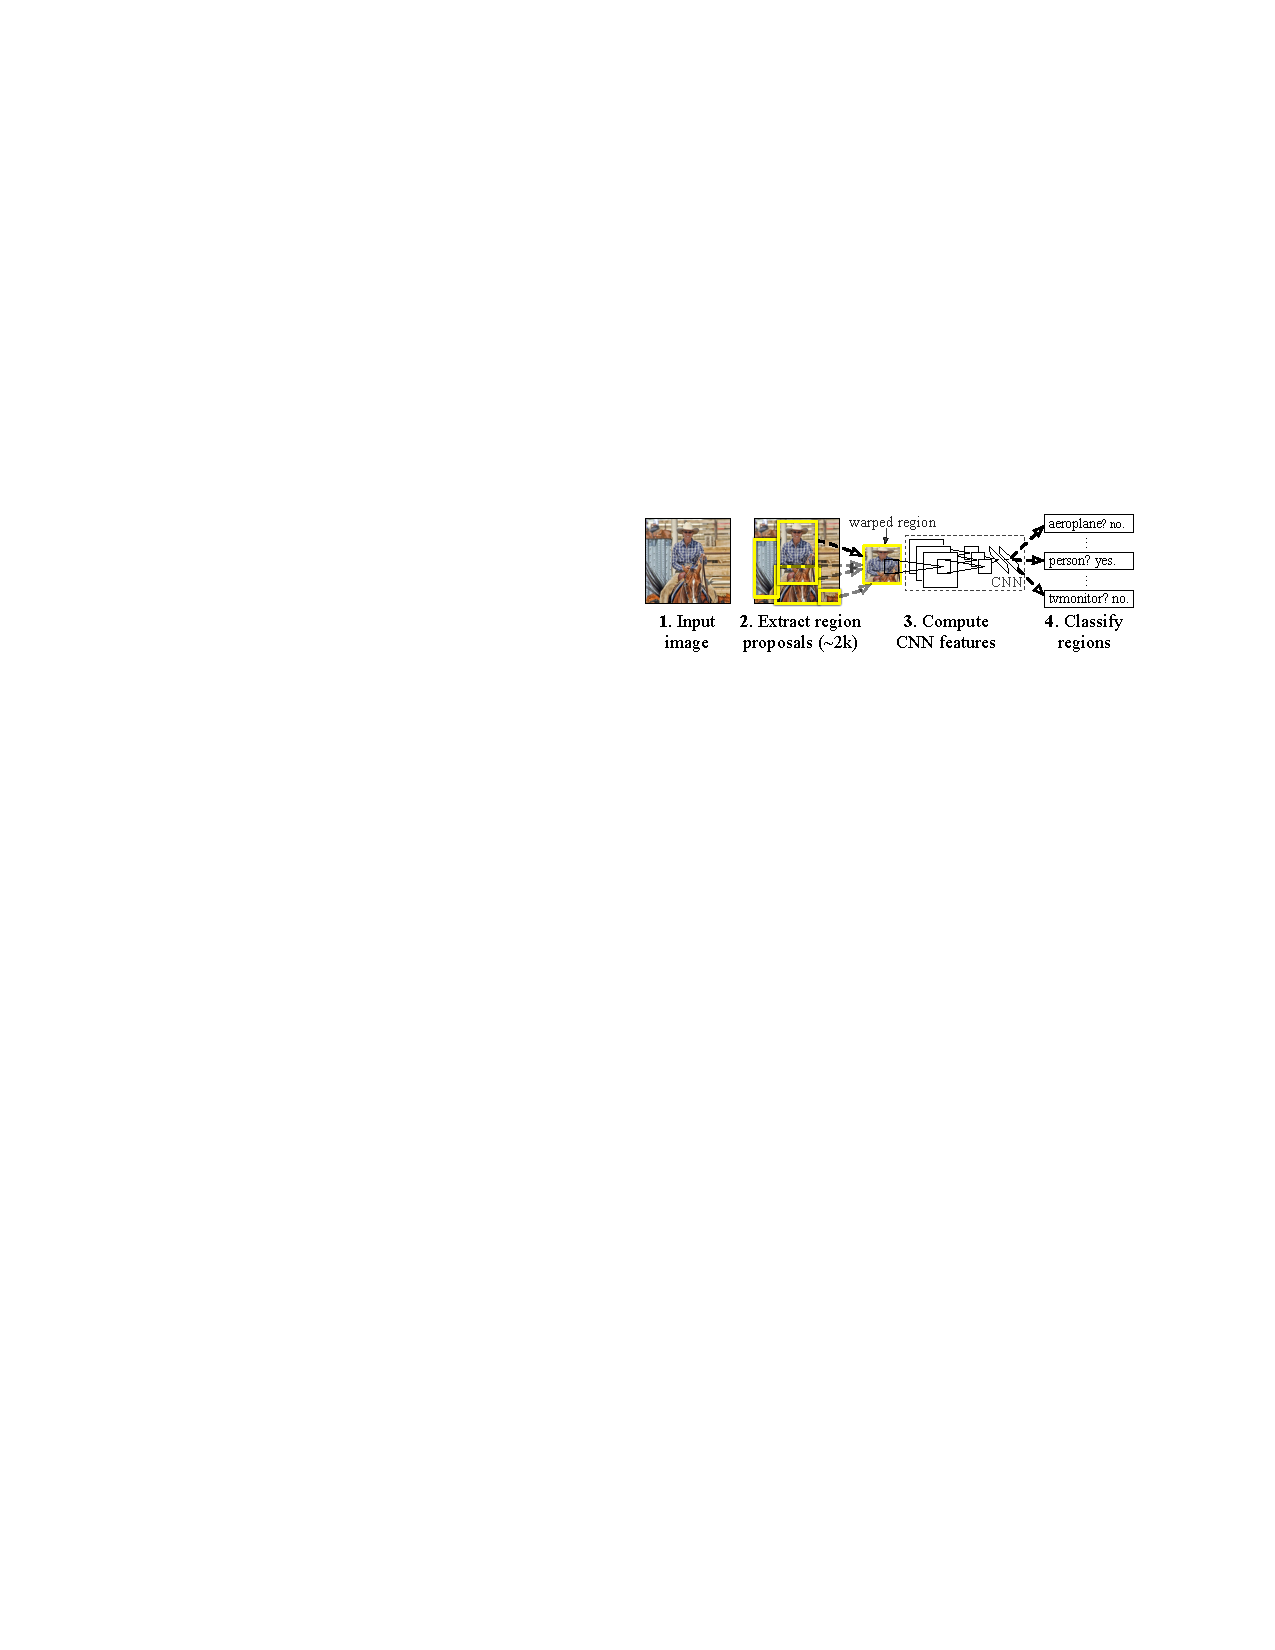
\includegraphics[width=0.8\textwidth]{../graphics/R-CNN.pdf}
   \caption{R-CNN strategy \cite{Girshick2014}}.
\end{figure}
\begin{itemize}
	\item Starting from region proposals (by any method): $\sim 2000$ regions). 
	\item Warping / Cropping of the selected regions into fixed resolution and extraction of a 4096-dimensional feature vector with a pretrained CNN. 
	\item Classification with SVM (object types and background). 
	\item Adjustment by bounding box regression
	\item Filtering with greedy non-maximum suppression (NMS): removal of regions with low overlap with a single object. 
\end{itemize}
%\vspace{-.5cm}
\end{frame}

\begin{frame}{Drawbacks of R-CNN}
\begin{itemize}
\item Fixed input size for the CNN: distortion and rescaling of images is necessary.
\item Multi-stage pipeline (no end-to-end solution, which is globally optimal).
\item Training is expensive in space and time, mainly due to the separate feature extraction step. 
\item Computationally expensive at prediction time, as many (overlapping) regions need to be classified. 
\item Sub-optimal region proposal step.
\end{itemize} 
\end{frame}

\begin{frame}{Fast R-CNN}
\begin{figure}[htb]
   \centering
   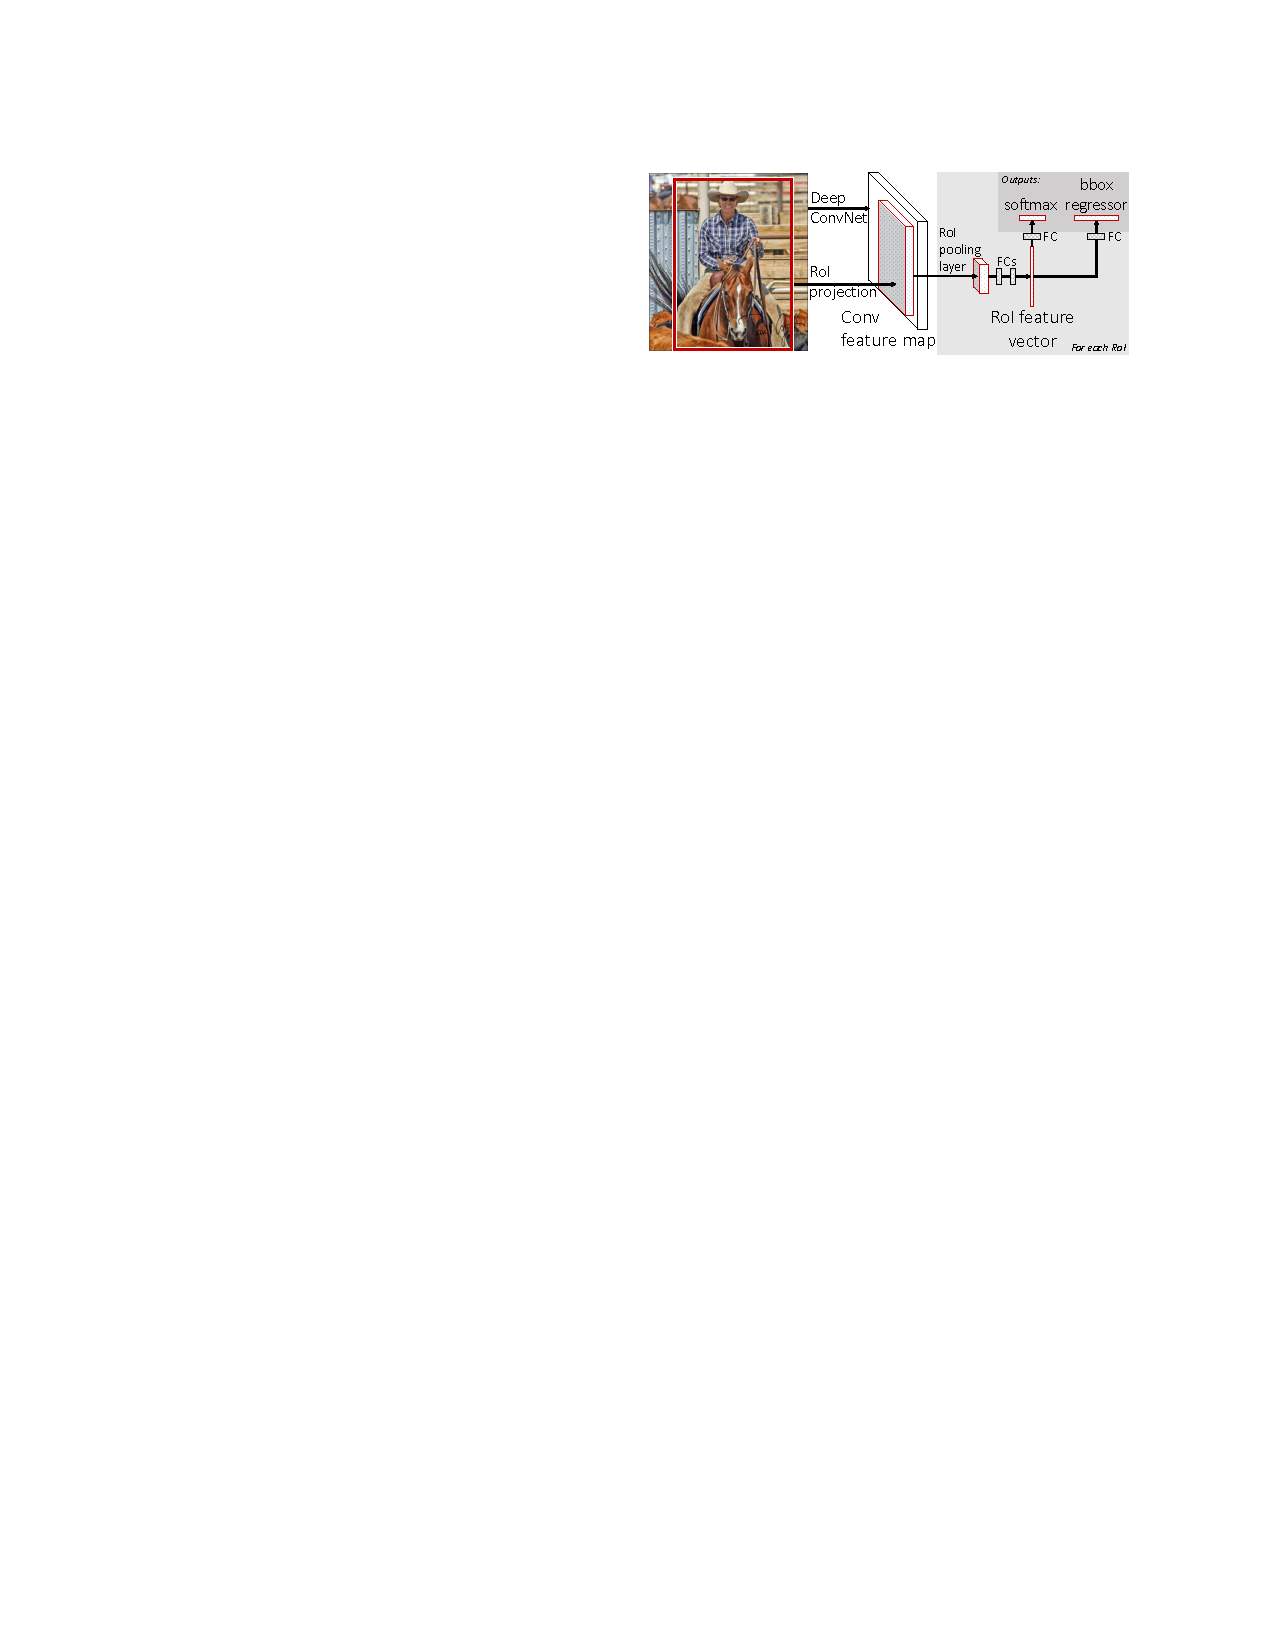
\includegraphics[width=0.8\textwidth]{../graphics/Fast_R-CNN.pdf}
   \caption{Fast R-CNN \cite{Girshick2015}}.
\end{figure}
\begin{itemize}
	\item The entire image is processed by a neural network: generation of feature maps.
	\item Region are proposed by some algorithm (as before).
	\item To each region, a ROI pooling layer is applied. 
\end{itemize}
%\vspace{-.5cm}
\end{frame}


\begin{frame}{Fast R-CNN: ROI pooling layer}
\begin{figure}[htb]
   \centering
   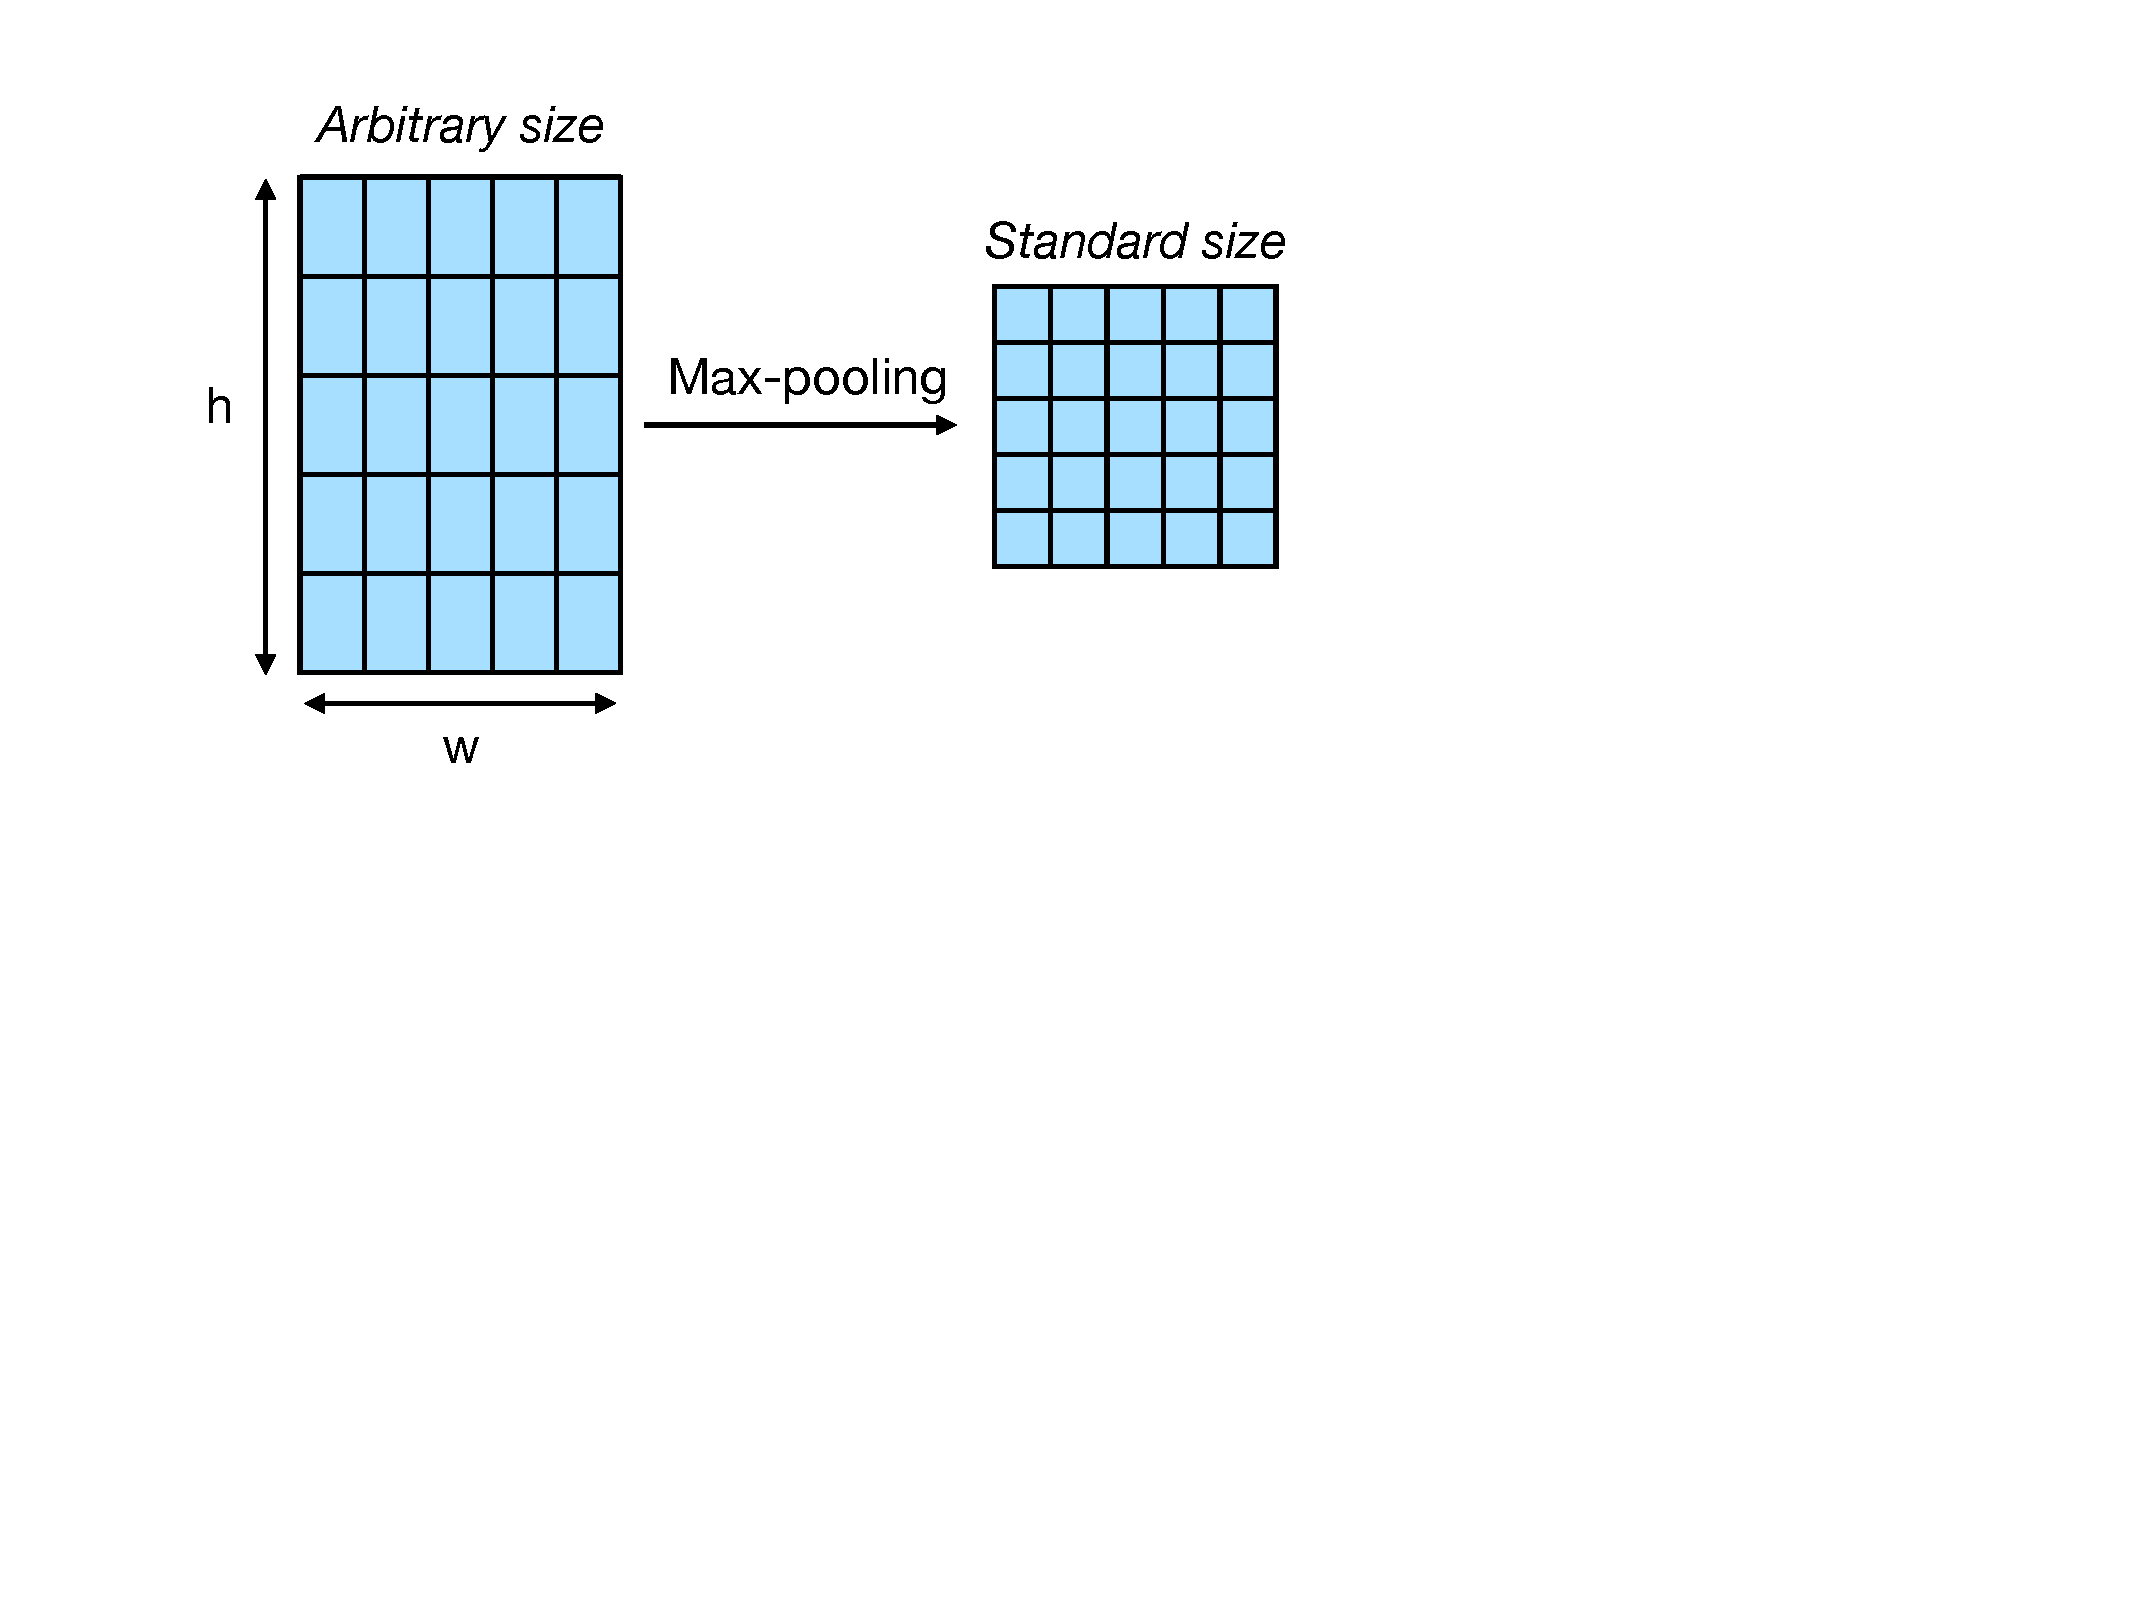
\includegraphics[height=0.4\textheight]{../graphics/ROI_pooling_layer.pdf}
   \caption{ROI pooling layer in Fast R-CNN}.
\end{figure}
\begin{itemize}
\item Each region of arbitrary size $w \times h$ is divided into $W \times H$ tiles. $W$ and $H$ are fixed, where as $w$ and $h$ are arbitrary.
\item For each tile, the maximum is calculated (max-pooling operation) in the feature map.
\item The output (fixed size) can then be processed by dense layers. 
\end{itemize}
%\vspace{-.5cm}
\end{frame}

\begin{frame}{Fast R-CNN: Output layer}
% \begin{figure}[htb]
%    \centering
%    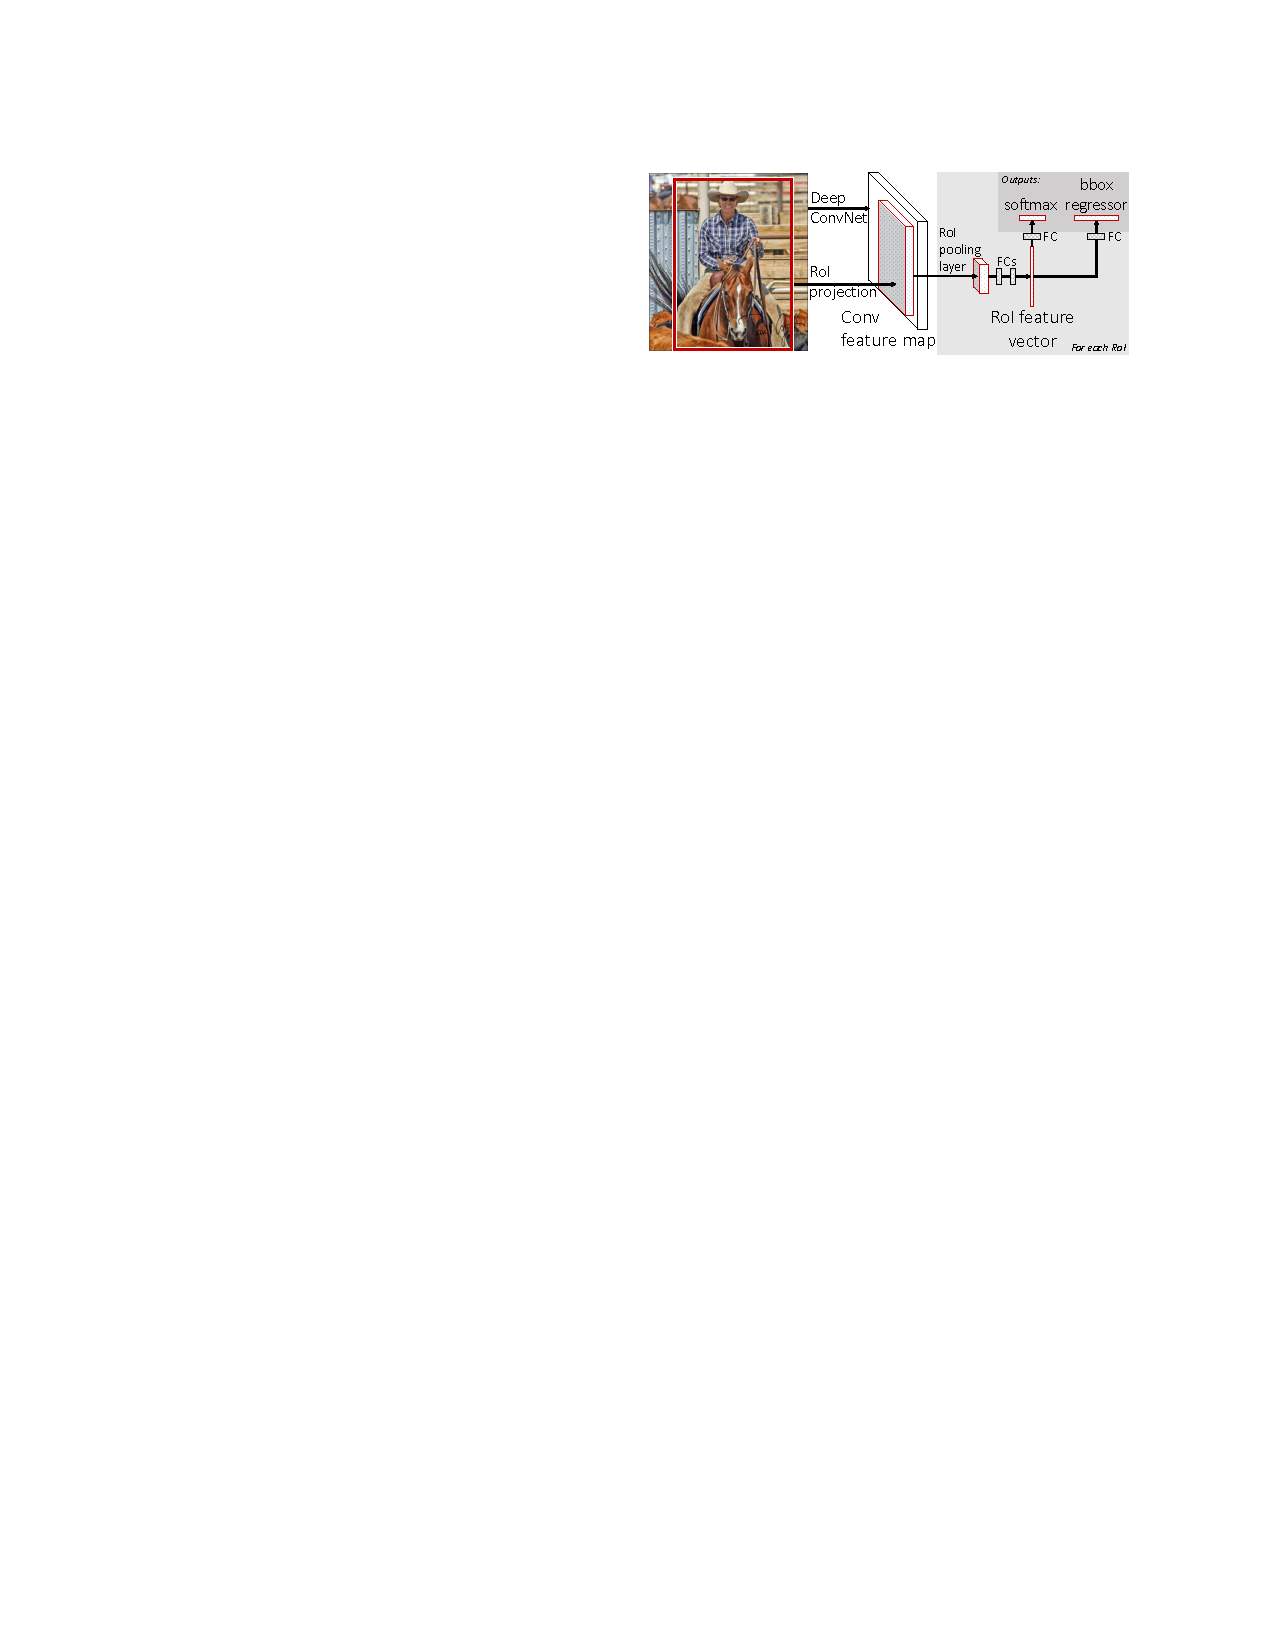
\includegraphics[width=0.8\textwidth]{../graphics/Fast_R-CNN.pdf}
%    \caption{Fast R-CNN \cite{Girshick2015}}.
% \end{figure}
\begin{itemize}
\item Two outputs:
\begin{itemize}
	\item Classification output (with a standard softmax layer)
	\item Bounding box regression: prediction of position and extension offsets with respect to the original region proposal. 
\end{itemize}
\item The loss has thus two components: $\loss_{class}$ which is the standard cross-entropy loss and $\loss_{loc}$, the localization loss ($\loss_1$ loss of the offsets with respect to the proposed regions).
% , i.e. for each sample we have a loss:
% \begin{equation*}
% \loss = - \sum_k y_k \log(\hat{y}_k) + \lambda[y \geq 1] \sum_{j \in \{x,y,w,h\}} \loss_1(v^k_j - \hat{v^k}_j)
% \end{equation*}
% where $v$ is the offset relative to a region proposal. 
\item During training, the batch is constructed from many objects drawn from very few images. Feature maps do then not need to be recalculated. 
\item For the prediction, each class gets its own region proposal, that is processed individually with non-maxima suppression. 
\end{itemize}
\end{frame}

% \begin{frame}{Fast R-CNN}
% \begin{itemize}
% \item Fast
% \end{itemize}
% \end{frame}

\begin{frame}{Faster R-CNN: motivation}
\begin{itemize}
	\item Fast R-CNN solves nearly all problem of R-CNN, and is end-to-end given a set of region proposals.
	\item The problem is that we still need to make region proposals to start with (time-consuming and two-stage algorithm).
	\item Faster R-CNN \cite{Ren2017} trains a network called Region Proposal Network (RPN) to overcome this issue.
\end{itemize}
\end{frame}

\begin{frame}{Faster R-CNN: Idea}
\begin{figure}[htb]
   \centering
   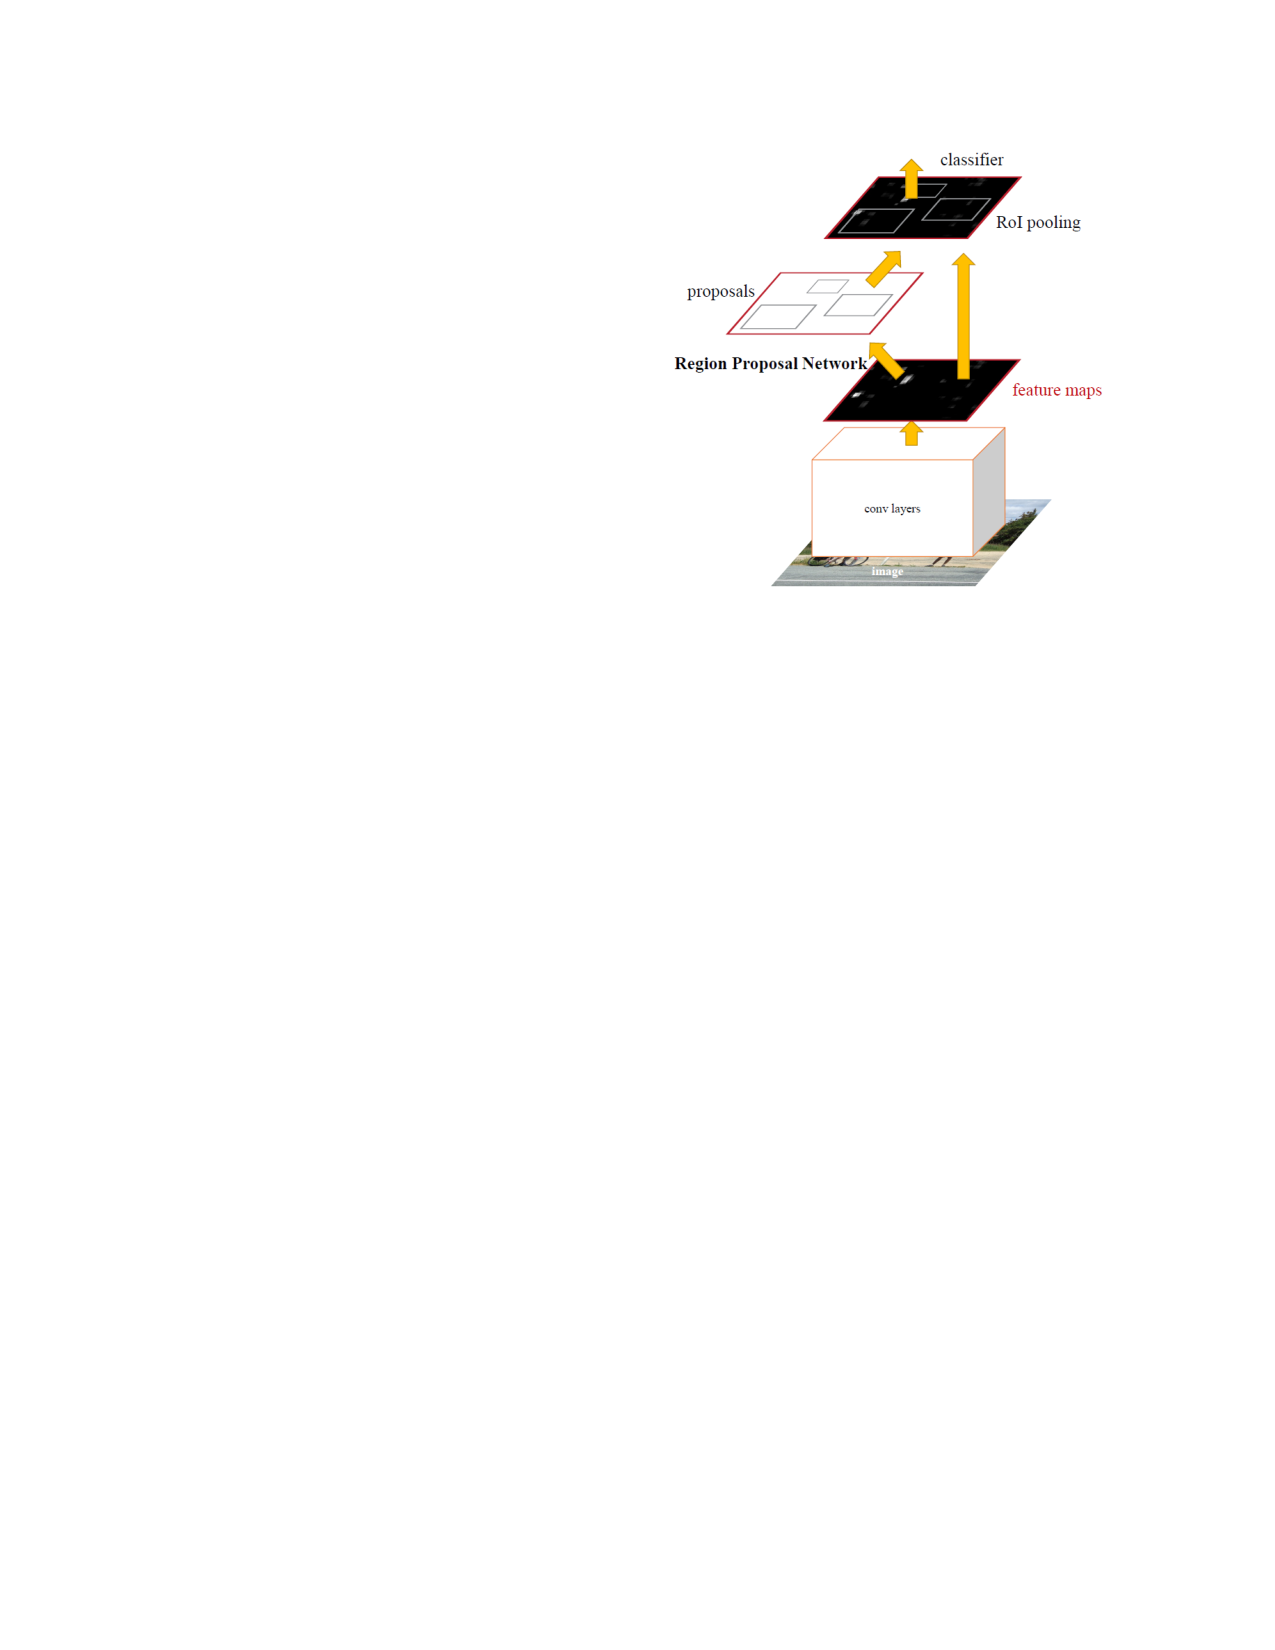
\includegraphics[width=0.4\textheight]{../graphics/Faster_R-CNN2.pdf}
   \caption{Faster R-CNN \cite{Ren2017}}.
\end{figure}
The idea is to share convolutional feature maps at test-time, i.e. to use the CNN feature maps calculated for the entire image for both region proposal and object classification \cite{Ren2017}. 
\end{frame}

\begin{frame}{Faster R-CNN: shared layers}
\begin{figure}[htb]
   \centering
   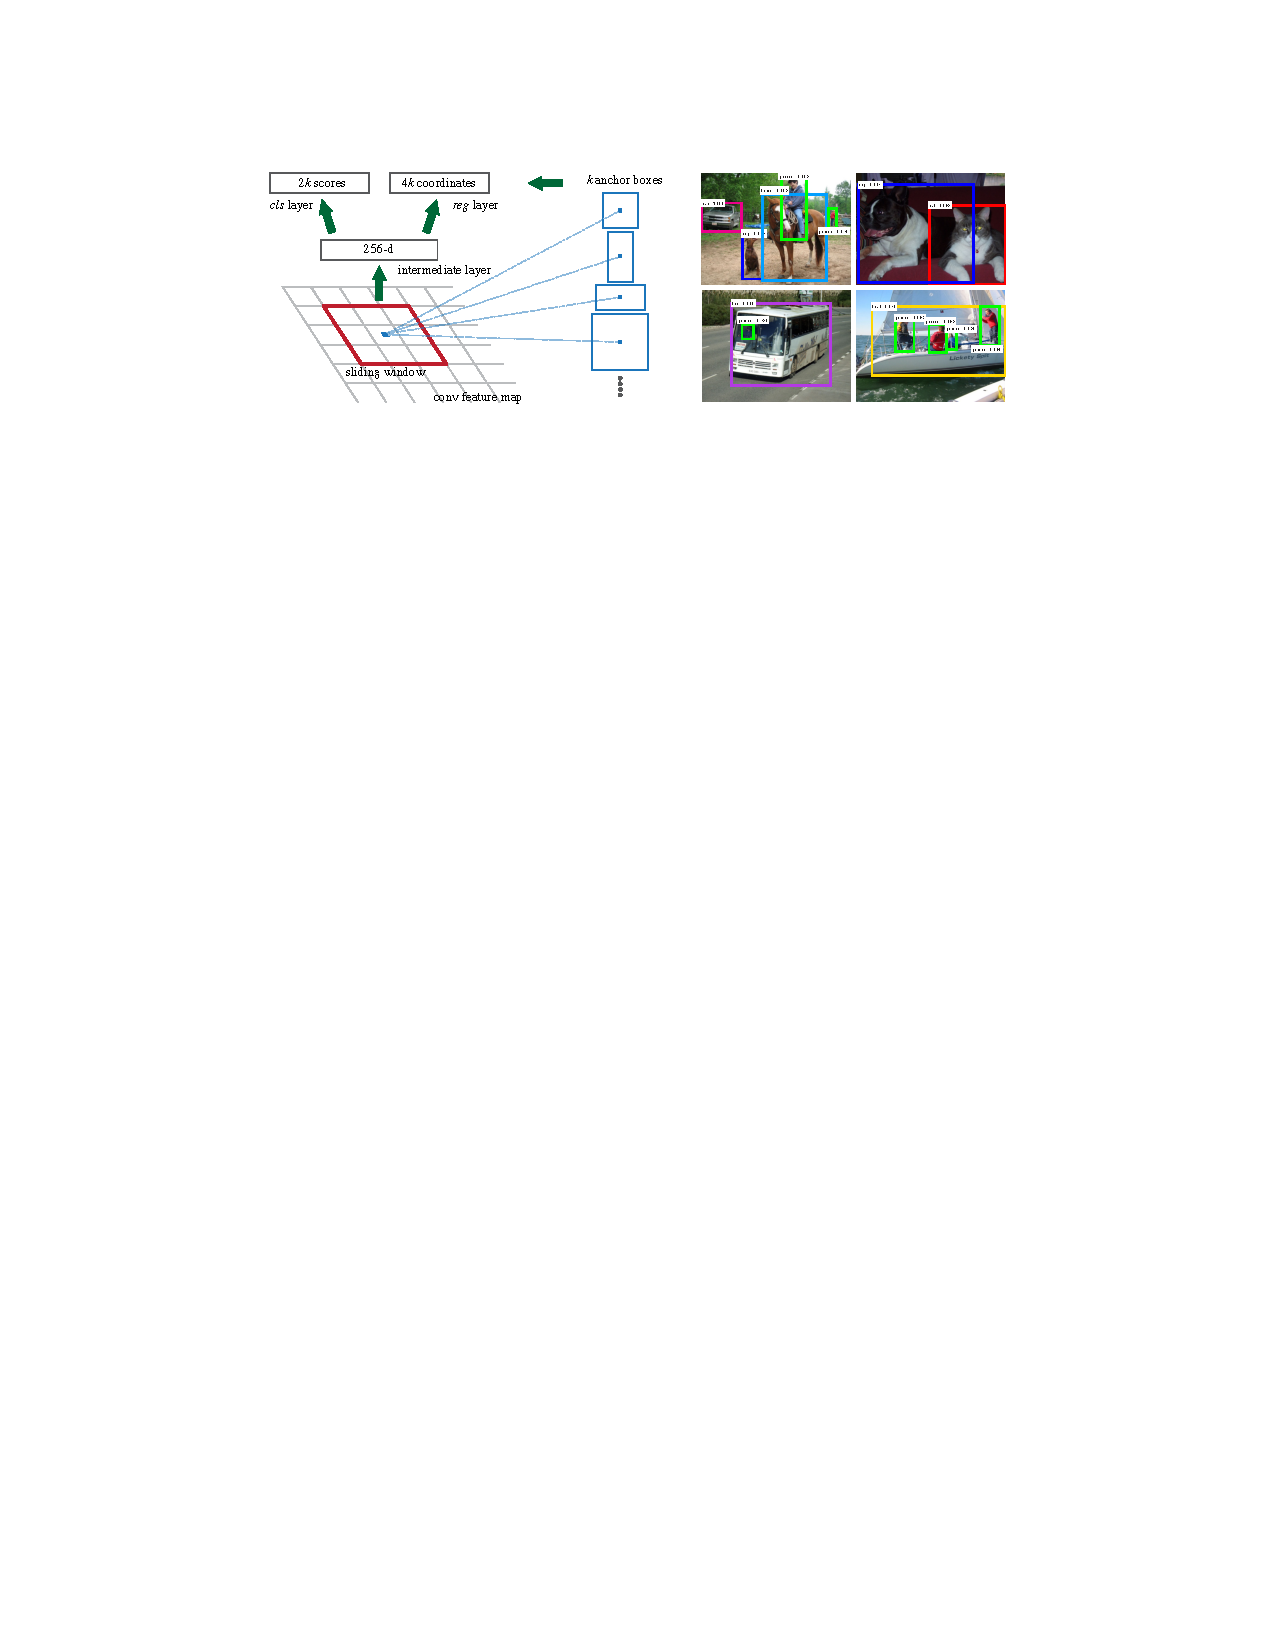
\includegraphics[width=0.8\textwidth]{../graphics/Faster_R-CNN.pdf}
   \caption{Faster R-CNN \cite{Ren2017}}.
\end{figure}
\begin{itemize}
\item First, we run the image through convolutional layers of a CNN and obtain feature maps that will serve both the region proposal and the object classification. 
\item We now "slide" a small $n \times n$ network over the common feature map. In practice, this is implemented as a convolutional layer, followed by $1D$-convolutions. 
\item The size can be relatively small (in \cite{Ren2017}, it is $3 \times 3$); the receptive field is much larger. 
% , that outputs both scores (object yes/no) and regression offsets defining the bounding box. 
% \item The size can be relatively small (in \cite{Ren2017}, it is $3 \times 3$); the receptive field is much larger. 
%\item The size of the window needs to be chosen such that the receptive field is larger than all regions in the ground truth. 
\end{itemize}
\end{frame}

\begin{frame}{Faster R-CNN: Region proposal network (RPN)}
\begin{figure}[htb]
   \centering
   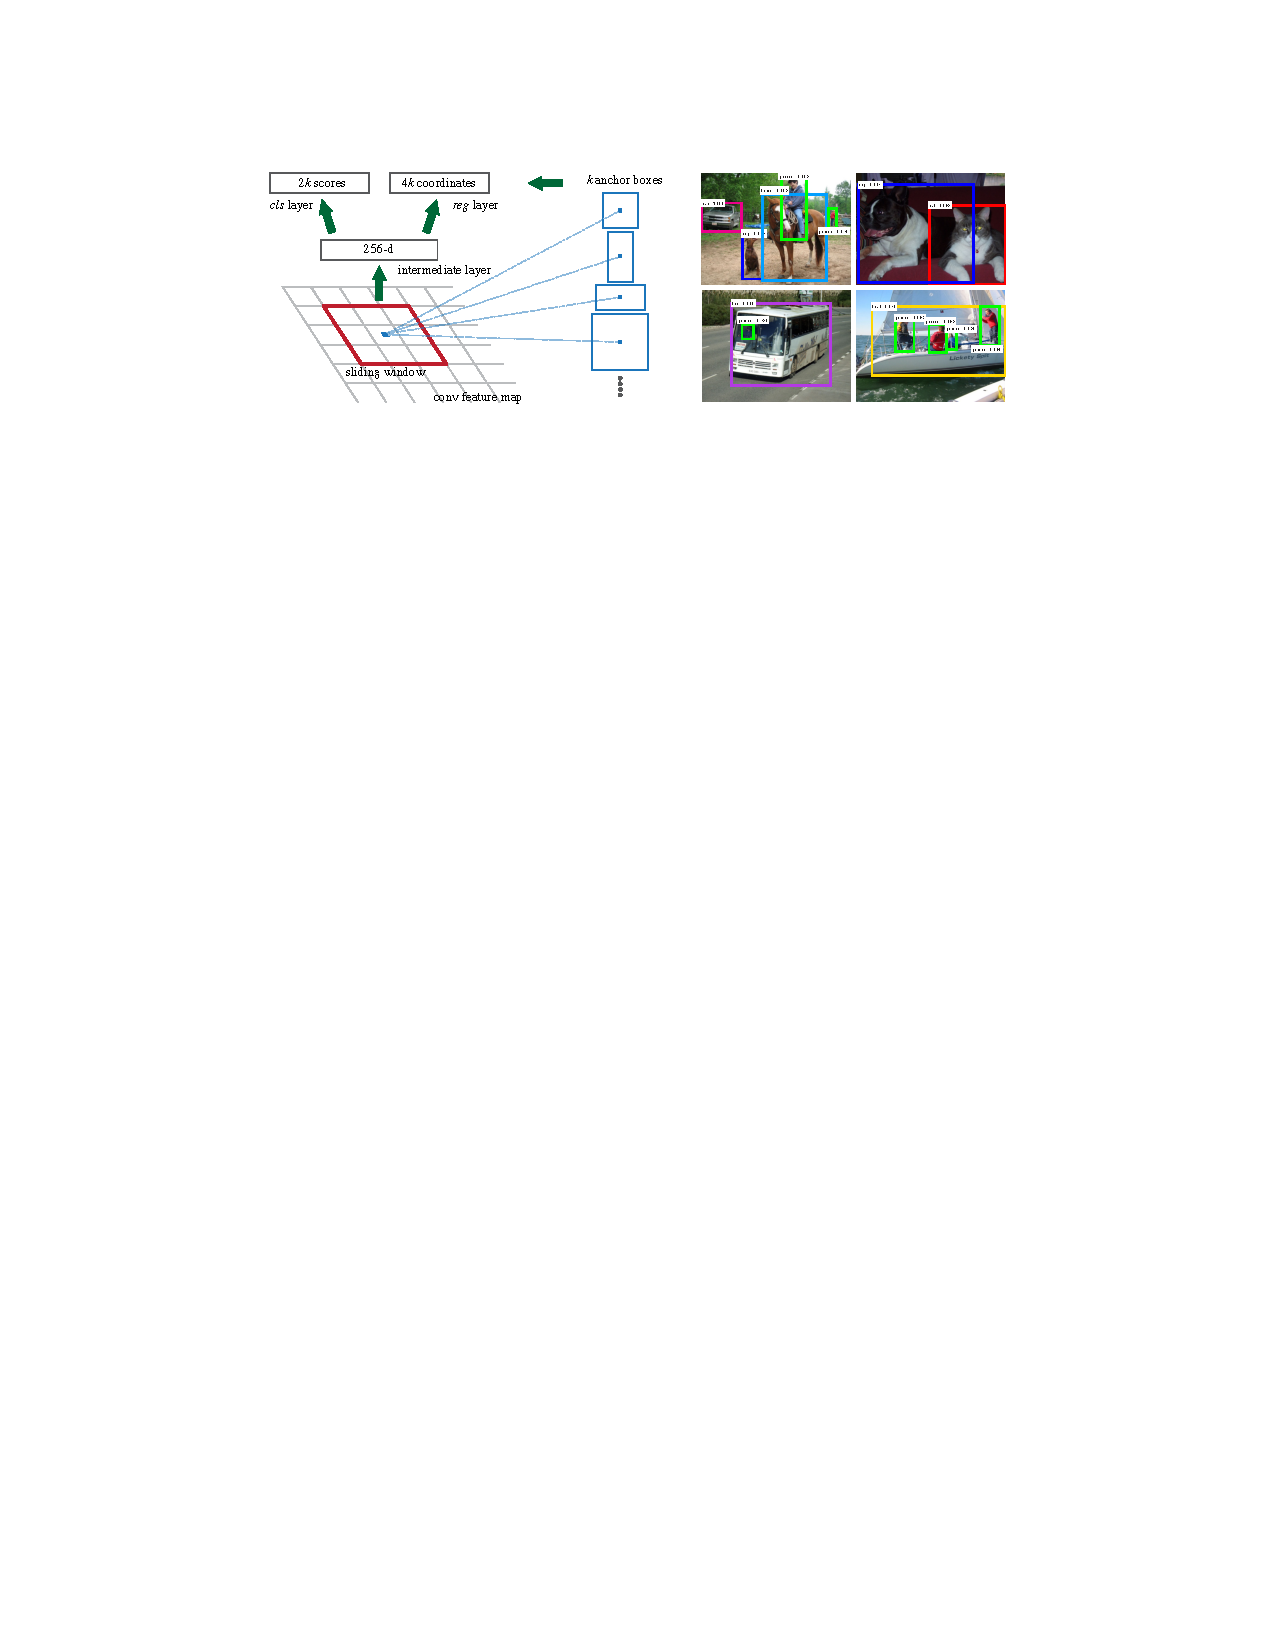
\includegraphics[width=0.8\textwidth]{../graphics/Faster_R-CNN.pdf}
   \caption{Faster R-CNN \cite{Ren2017}}.
\end{figure}
\begin{itemize}
\item This small network completes the Region Proposal Network (RPN).
\item The RPN outputs a set of rectangular object proposals, each with an objectness score.
\item For this, we define $k$ anchor regions (defined by scale and aspect ratio) at each sliding-window location.
\end{itemize}
\end{frame}

\begin{frame}{Faster R-CNN: Region proposal network (RPN)}
\begin{figure}[htb]
   \centering
   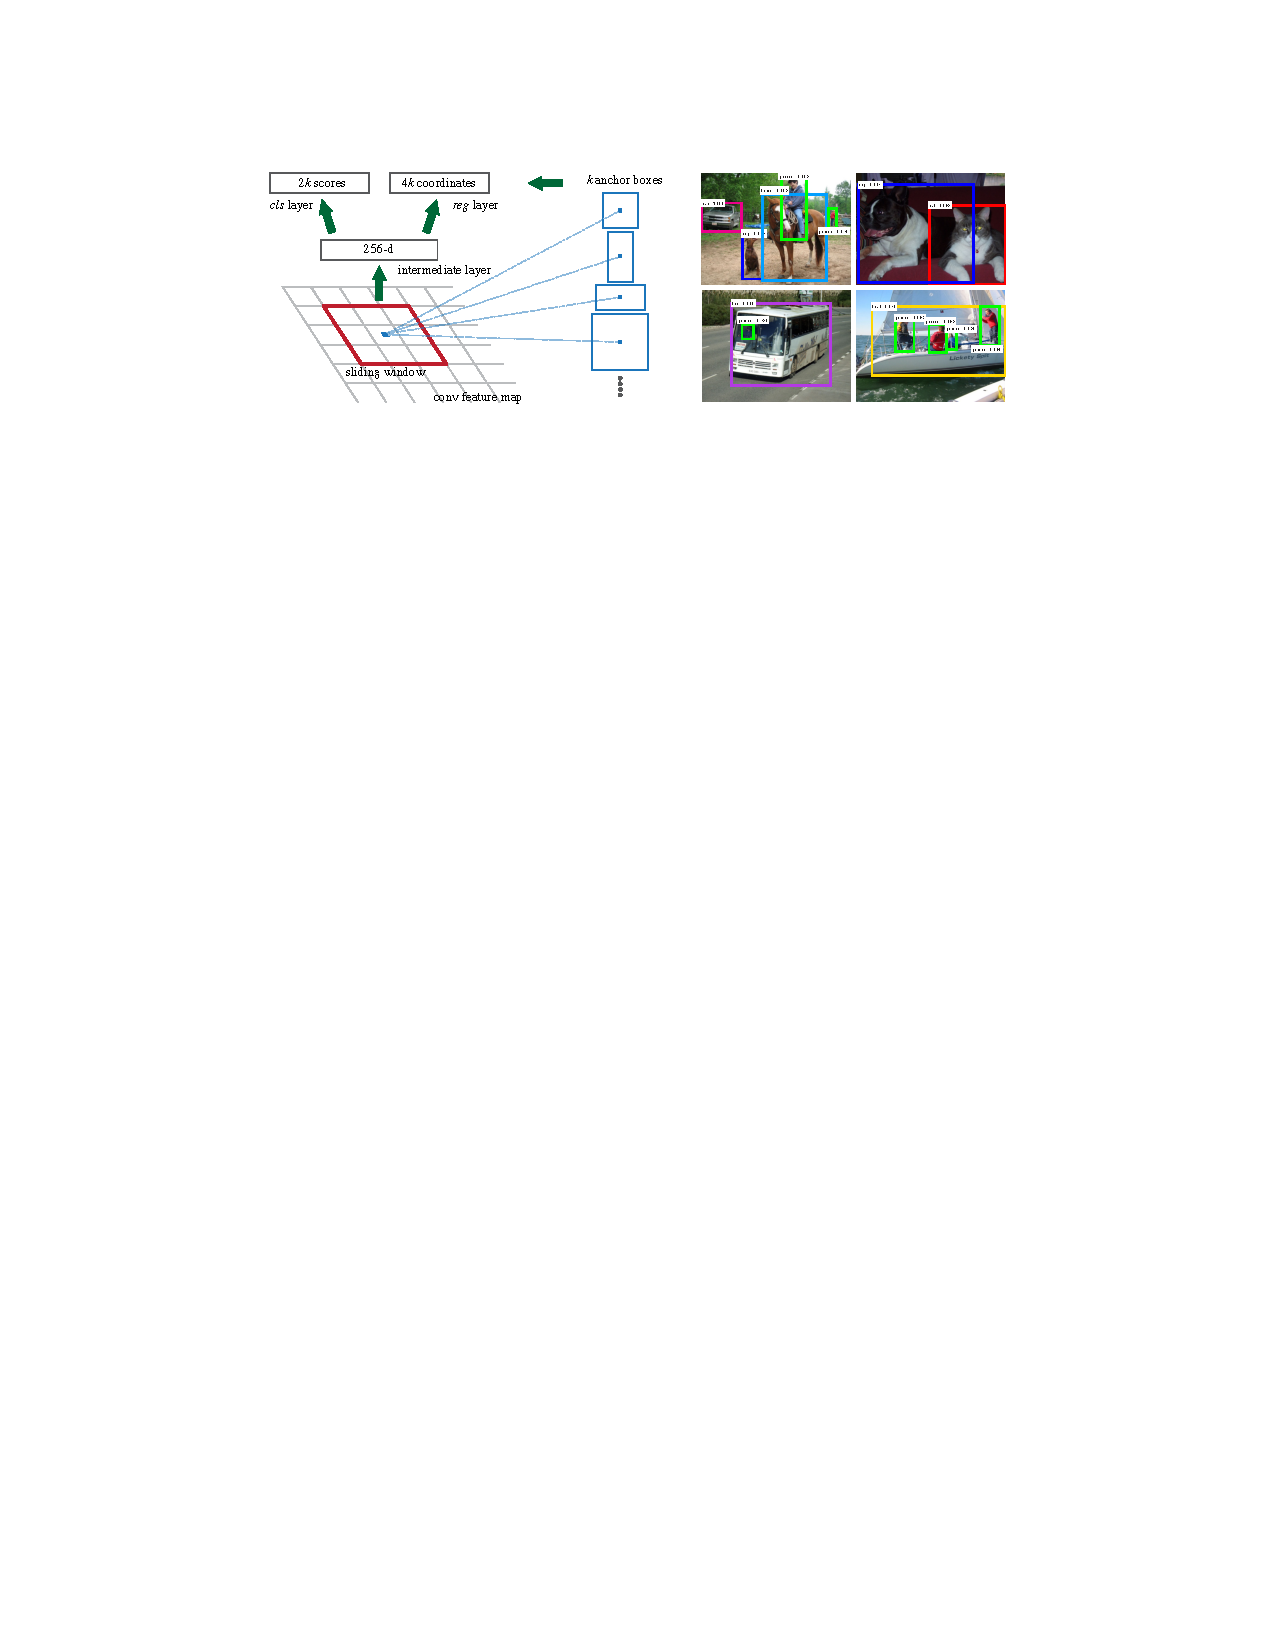
\includegraphics[width=0.8\textwidth]{../graphics/Faster_R-CNN.pdf}
   \caption{Faster R-CNN \cite{Ren2017}}.
\end{figure}
\begin{itemize}
\item For each sliding windows location and each of the $k$ anchors, we predict:
\begin{itemize}
   \item Objectness (object yes/no) of the anchor.
   \item Width, height and offset w.r.t. the anchor.
\end{itemize}
\item During training, an anchor is considered to be positive if the $IoU>0.7$ or if the $IoU$ is maximal among all anchors and none is larger than 0.7. Negative anchors have $IoU<0.3$. 
\end{itemize}
\end{frame}

% \begin{frame}{Faster R-CNN: Region proposal network (RPN)}
% \begin{figure}[htb]
%    \centering
%    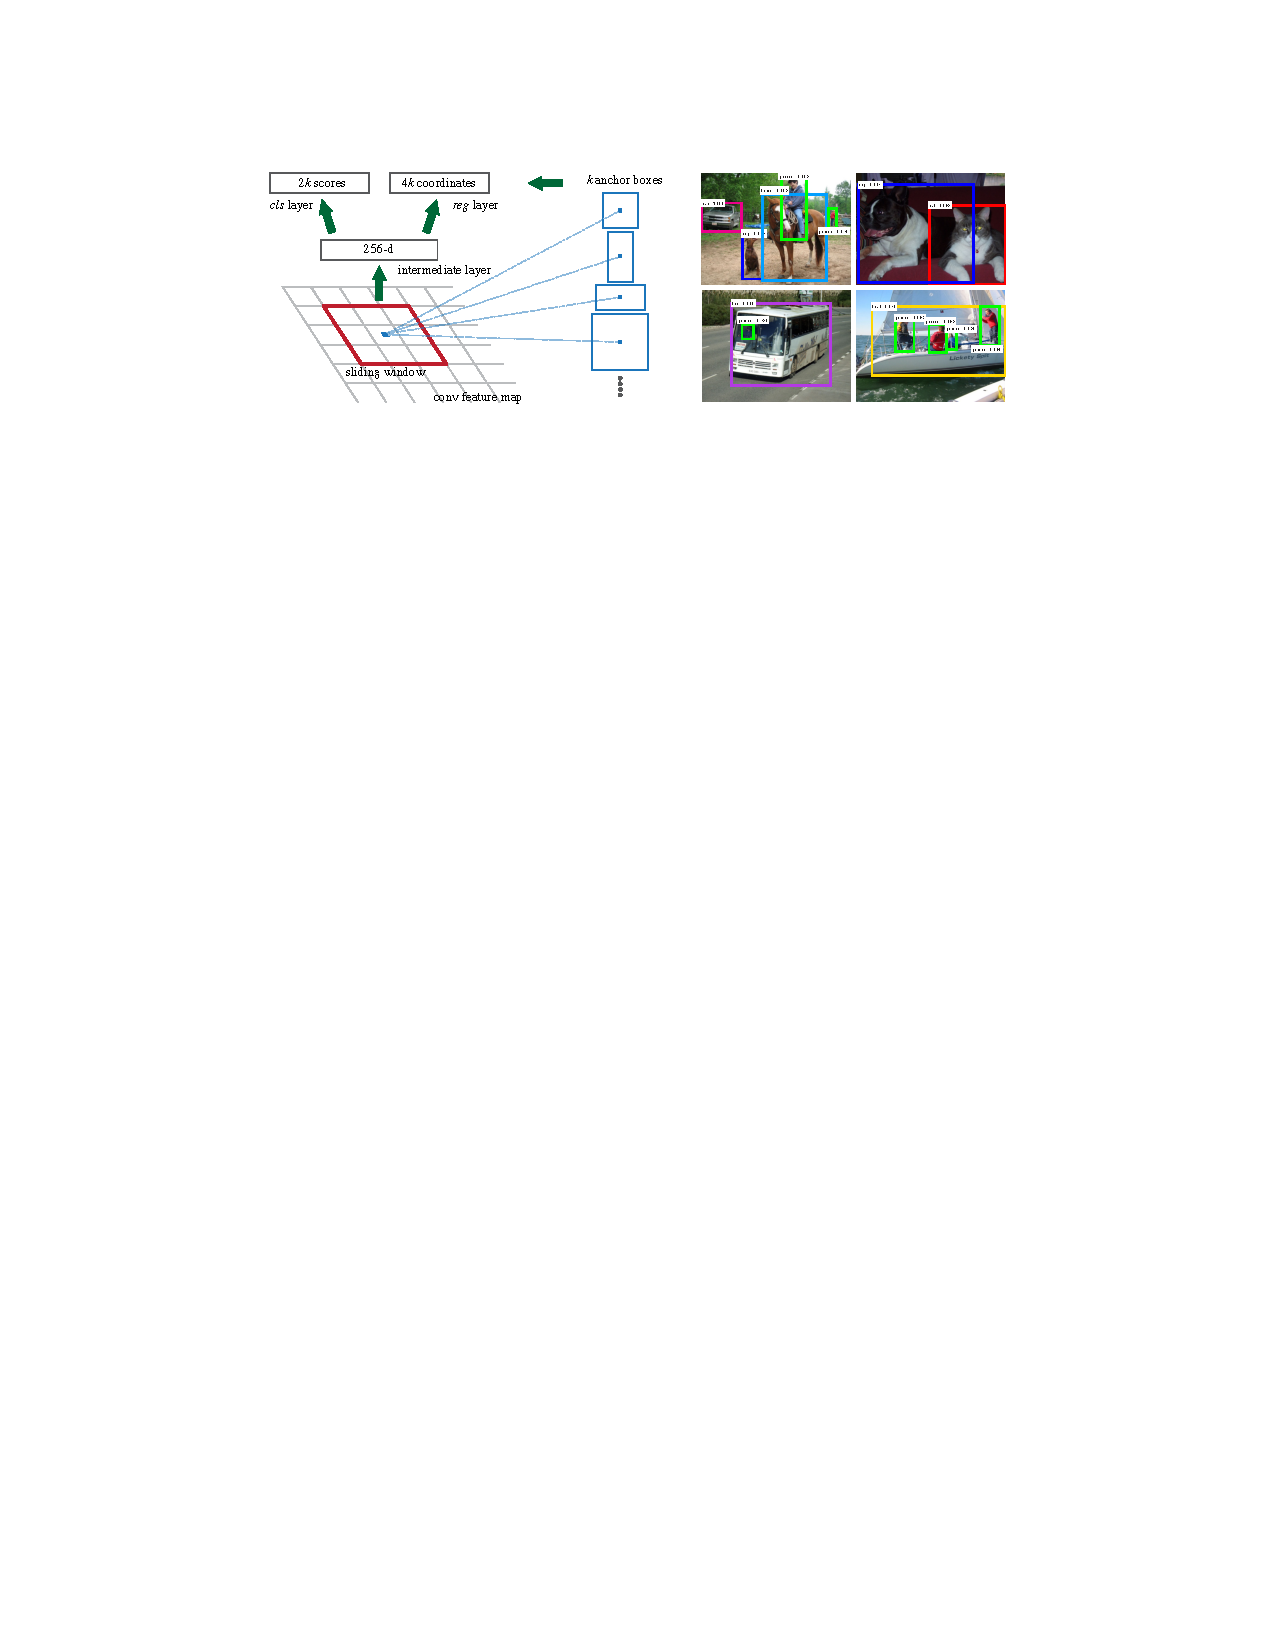
\includegraphics[width=0.8\textwidth]{../graphics/Faster_R-CNN.pdf}
%    \caption{Faster R-CNN \cite{Ren2017}}.
% \end{figure}
% \begin{itemize}
% \item A Region Proposal Network (RPN) takes an image as input and outputs a set of rectangular object proposals, each with an objectness score.
% \item We define $k$ anchor regions (defined by scale and aspect ratio).
% \item At each sliding-window location, we simultaneously predict $k$ region proposals from the $k$ anchor regions, for each we predict a score (object yes/no) and the box offsets.
% \end{itemize}
% \end{frame}

\begin{frame}{Faster R-CNN: Region proposal network (RPN)}
\begin{figure}[htb]
   \centering
   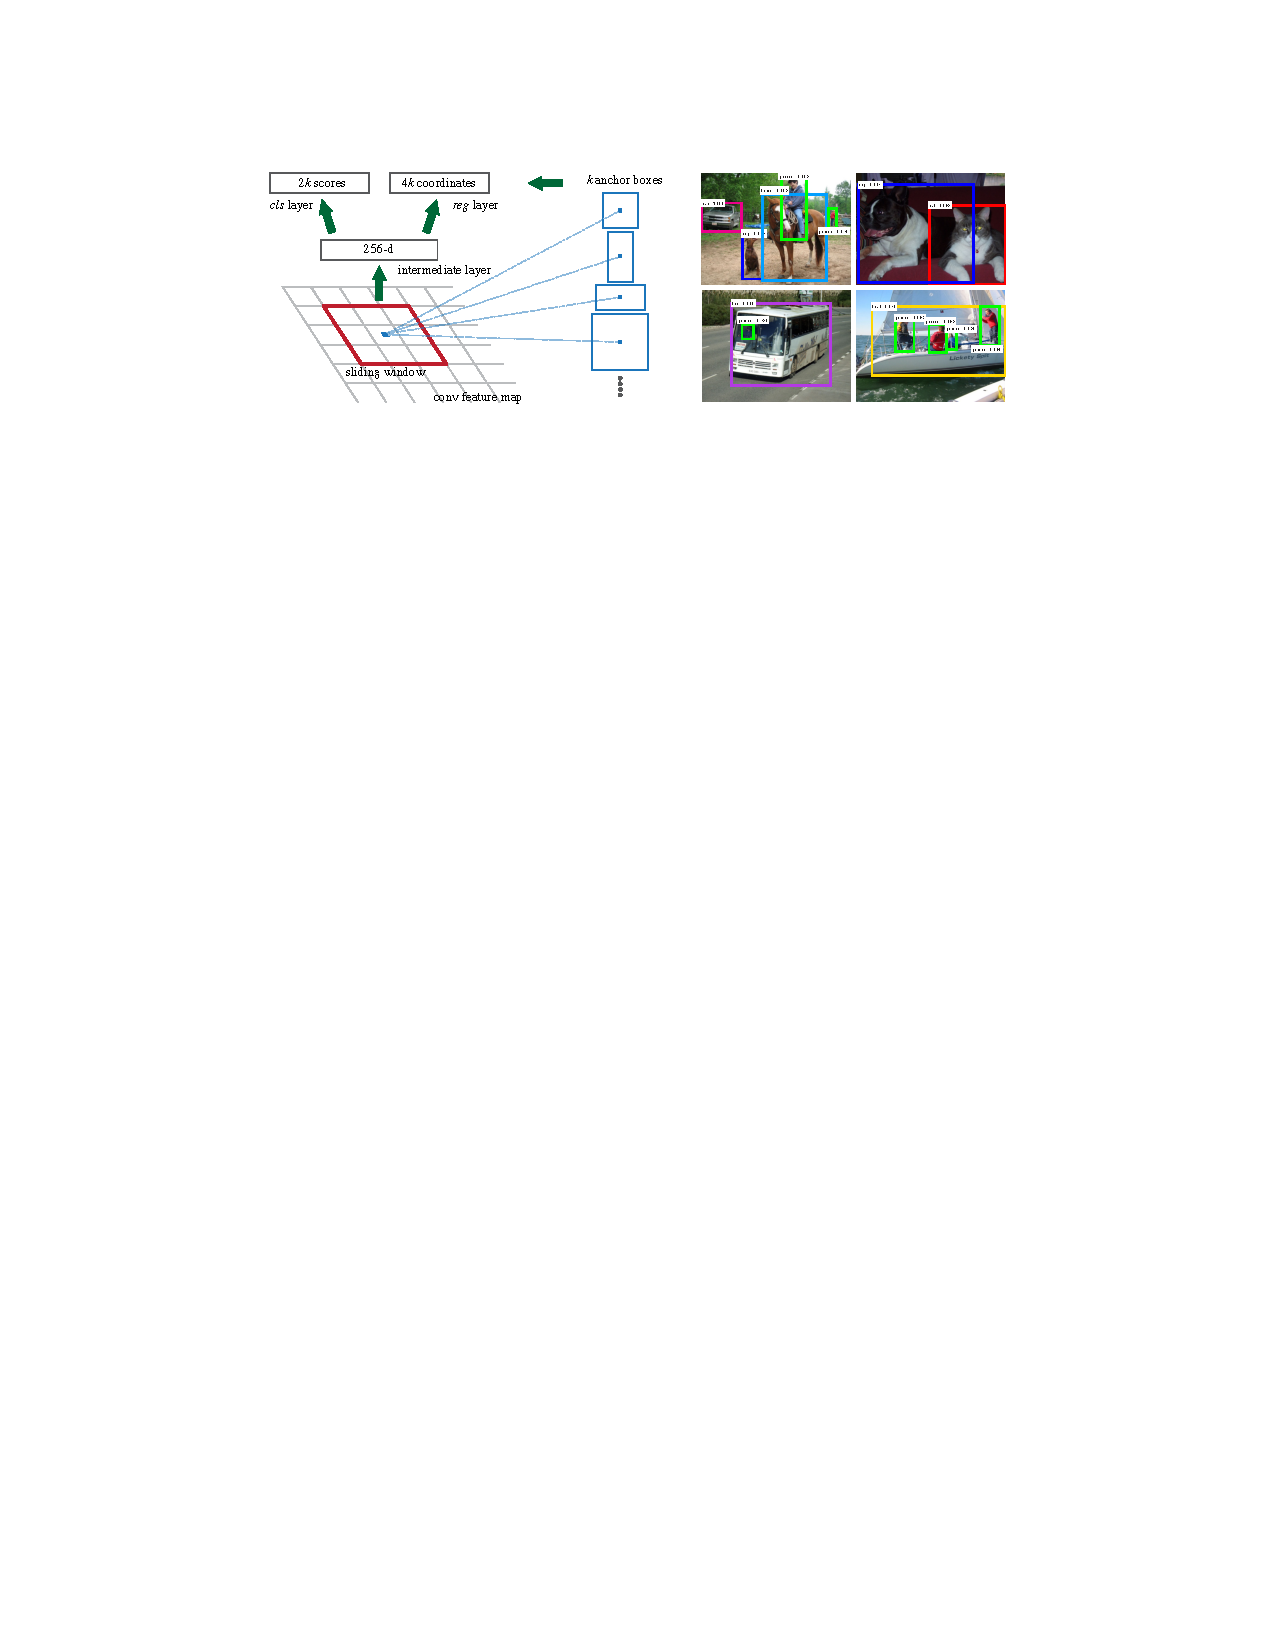
\includegraphics[width=0.8\textwidth]{../graphics/Faster_R-CNN.pdf}
   \caption{Faster R-CNN \cite{Ren2017}}.
\end{figure}
\begin{itemize}
\item We define a combined loss (as for Fast R-CNN), as sum of the classification loss and bounding box regression loss.
\item Classification loss: cross entropy for a binary classifier, indicating whether the region contains an object or not.
\item Regression loss compares for each region proposal its offsets to the anchors with the offsets of the ground truth box.
\end{itemize}
\end{frame}

\begin{frame}{Faster R-CNN: Training}
\begin{figure}[htb]
   \centering
   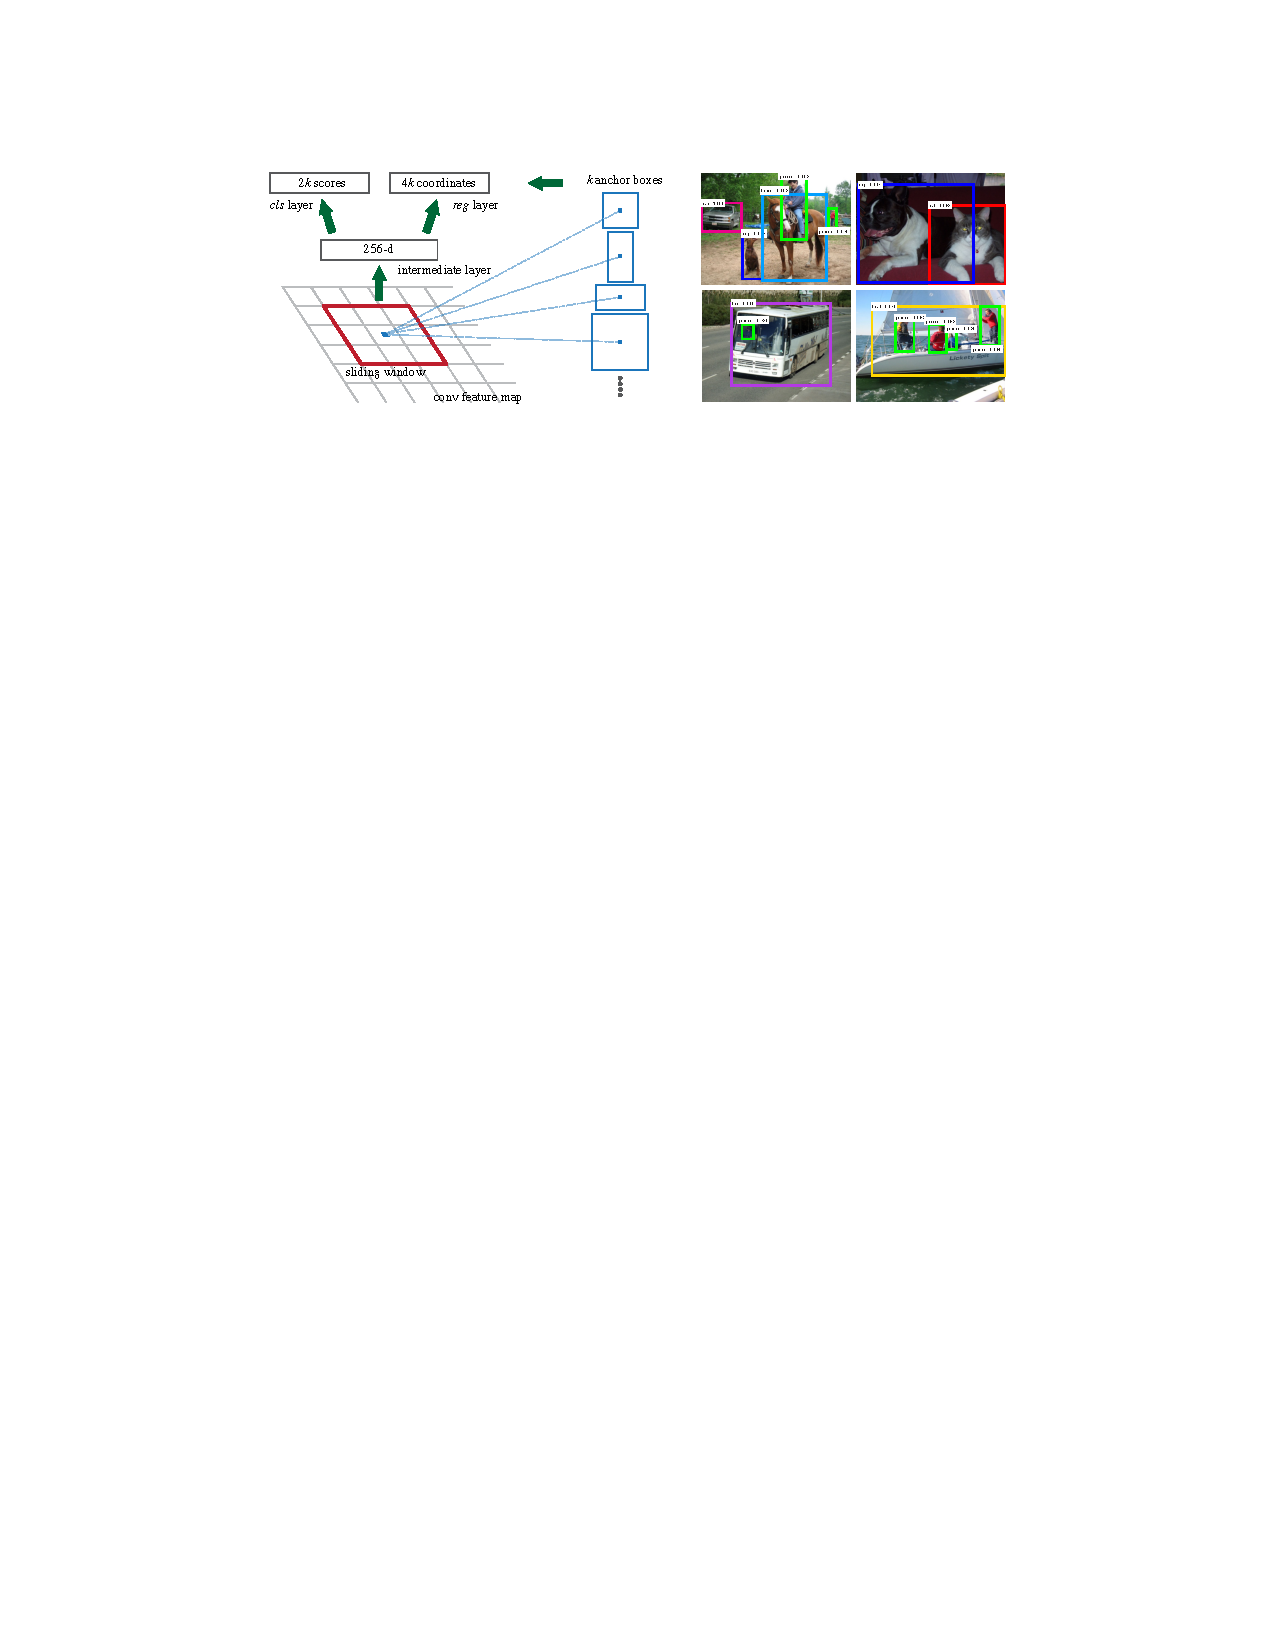
\includegraphics[width=0.8\textwidth]{../graphics/Faster_R-CNN.pdf}
   \caption{Faster R-CNN \cite{Ren2017}}.
\end{figure}
\begin{itemize}
\item We now simply apply a Fast R-CNN to the region proposals provided by the RPN.
\item The shared layers are trained in an alternating scheme.
\item After this initial training, the shared layers are frozen and the separate layers are trained end-to-end.
\end{itemize}
\end{frame}

\begin{frame}{YOLO: You only look once}
% \begin{figure}[htb]
%    \centering
%    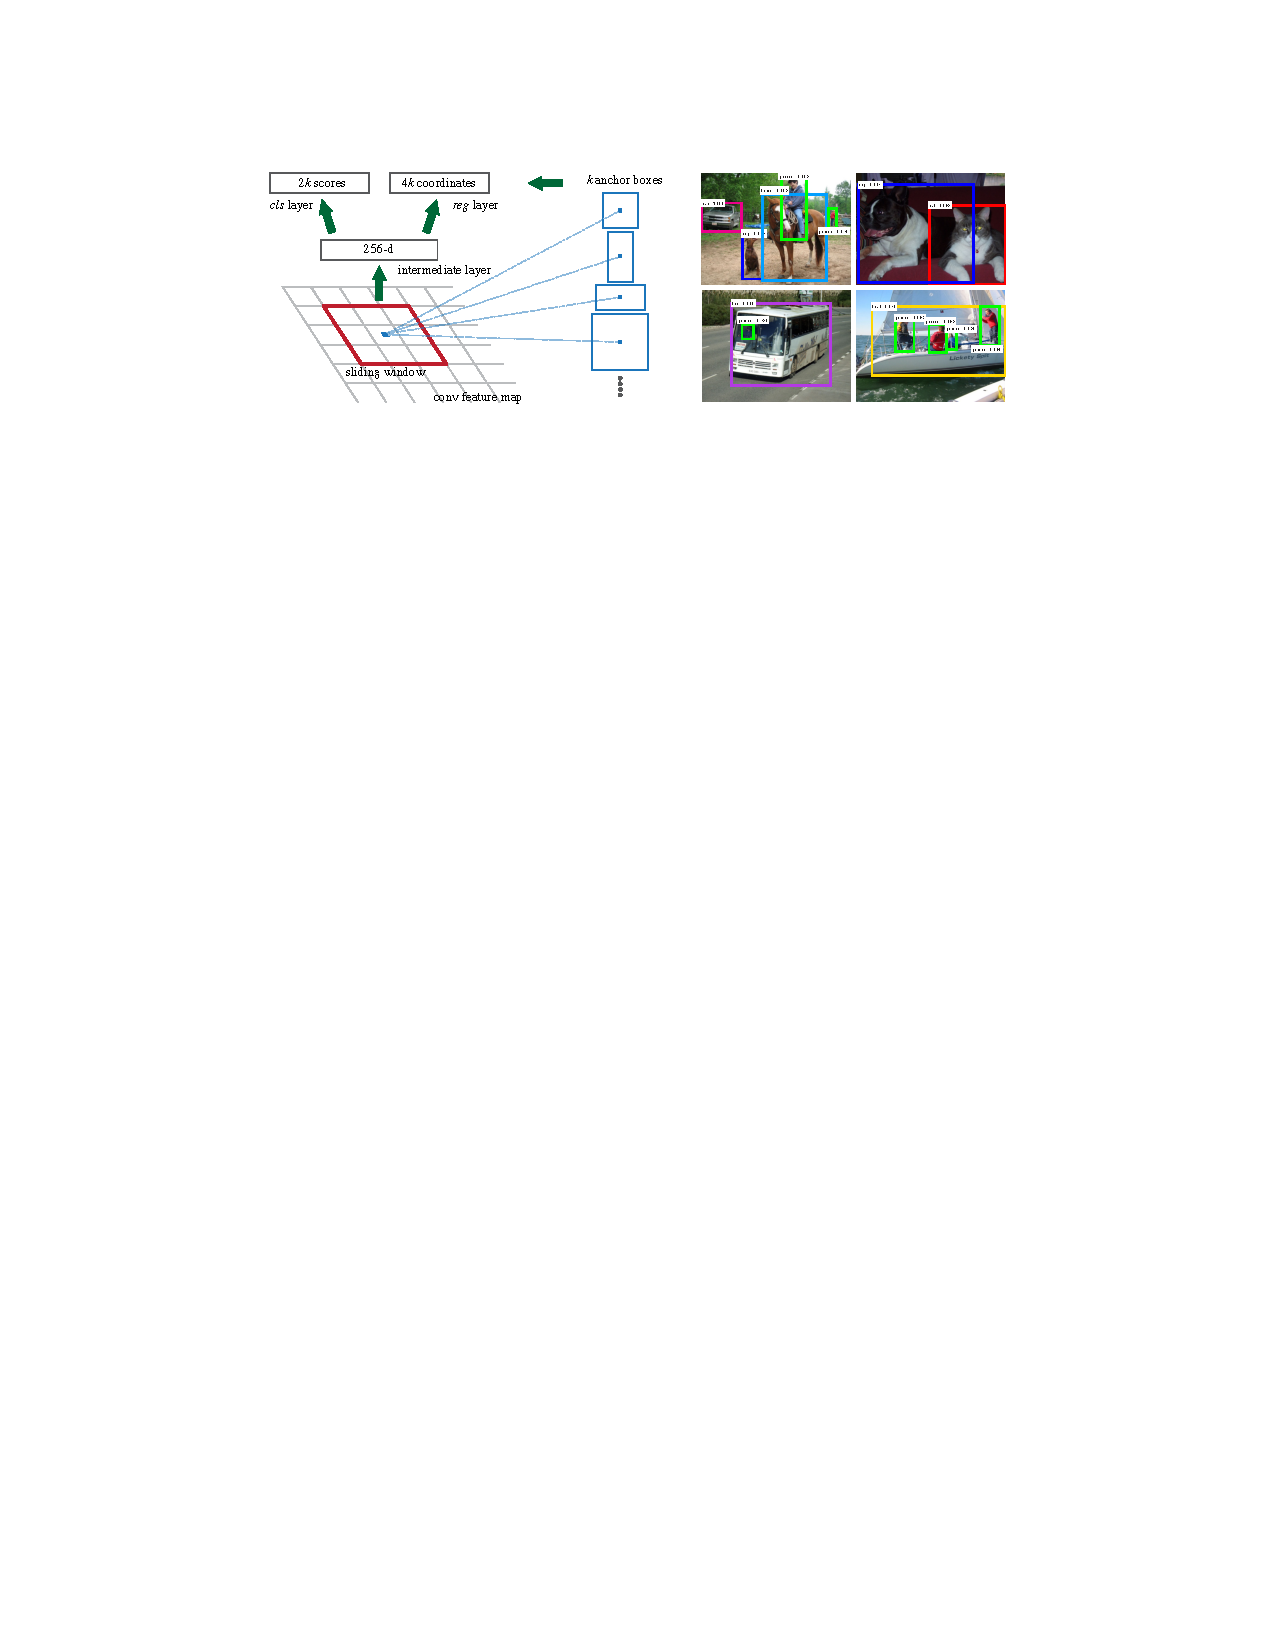
\includegraphics[width=0.8\textwidth]{../graphics/Faster_R-CNN.pdf}
%    \caption{Faster R-CNN \cite{Ren2017}}.
% \end{figure}
\begin{itemize}
\item Problem of most detection systems: 
\begin{itemize}
\item First: region proposals 
\item Second: classification of all region proposals individually
\item Consequently: the best performing methods are very slow and not applicable in real-time
\end{itemize}
\item YOLO \cite{Redmon2016}: end-to-end strategy that only uses one forward-pass of an image for object detection. 
\end{itemize}
\end{frame}

\begin{frame}{YOLO: principle}
\begin{figure}[htb]
   \centering
   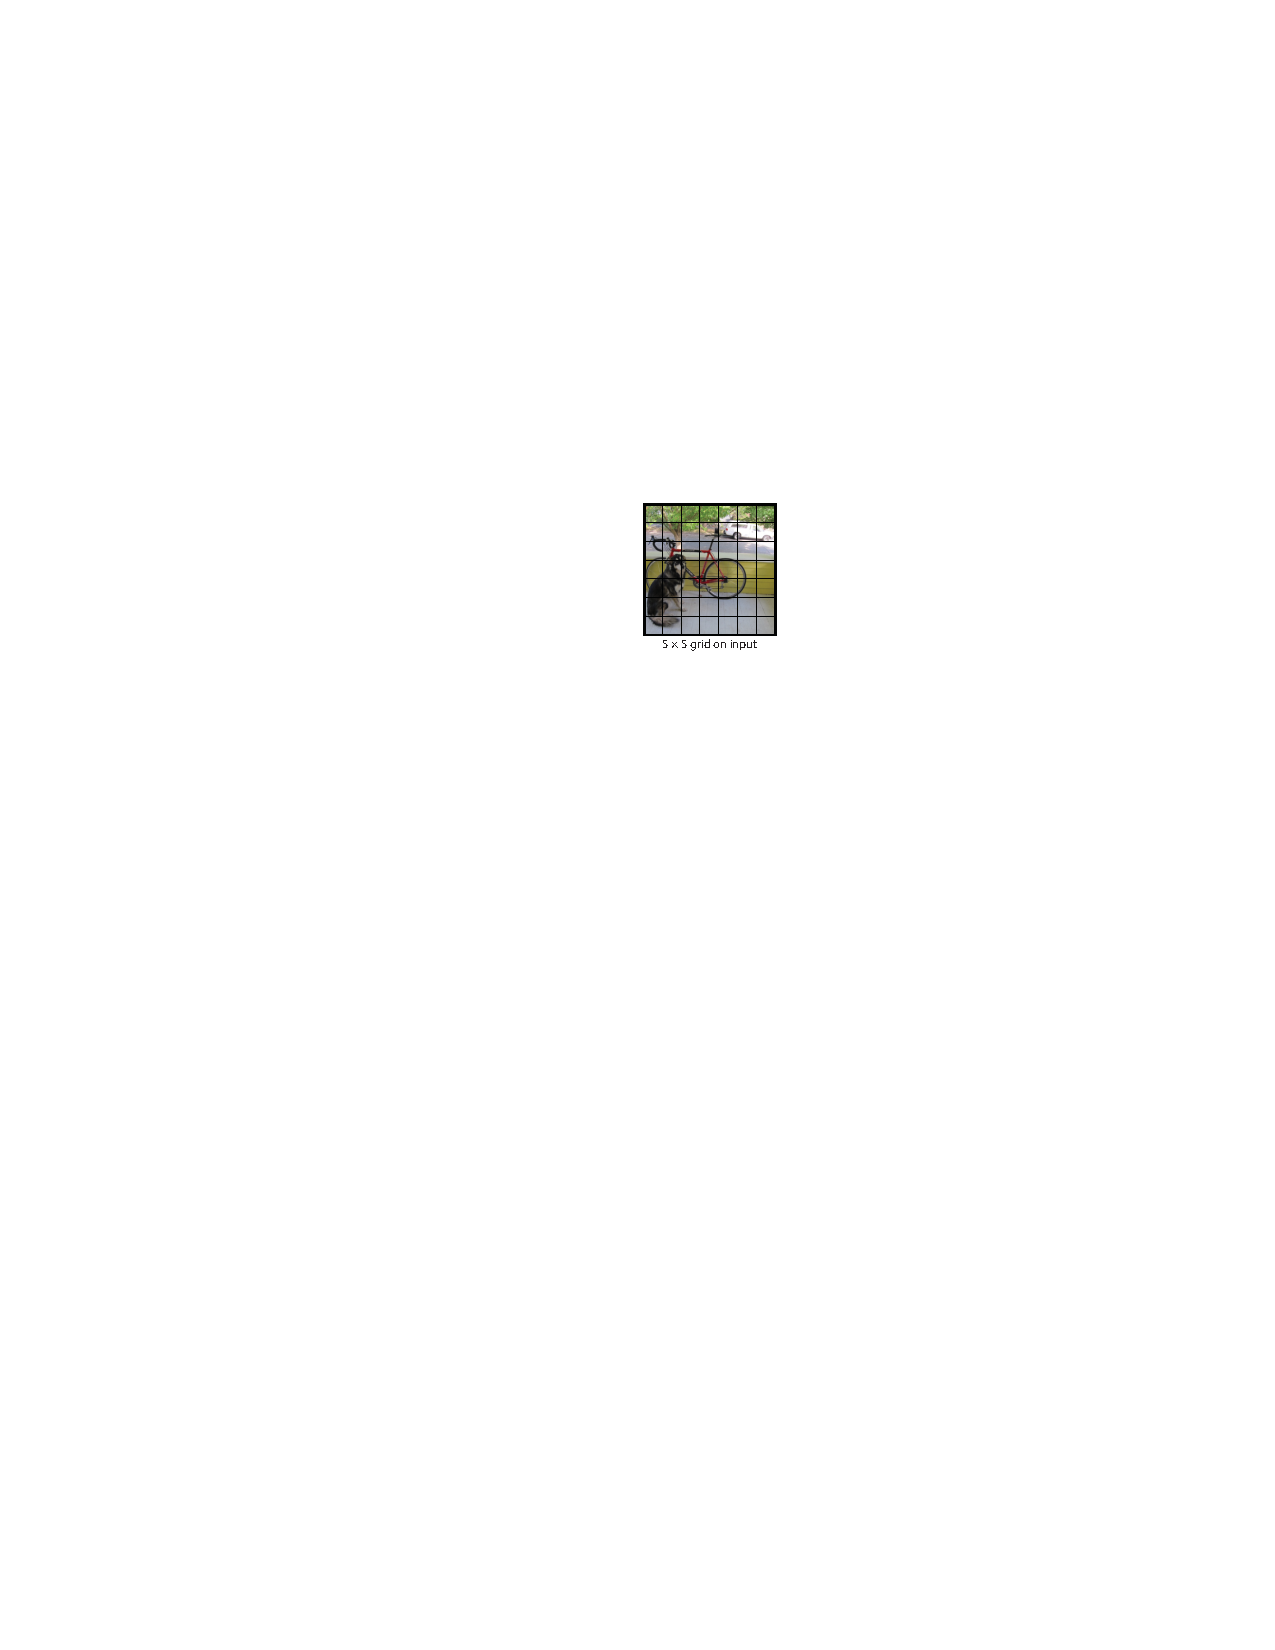
\includegraphics[height=0.4\textheight]{../graphics/YOLO_1.pdf}
   \caption{YOLO: the image is partitioned by an $S \times S$ grid.}
\end{figure}
\begin{itemize}
   \item First, the image is divided into a $S \times S$ grid of cells. 
   \item For each of these cells, we will then predict:
   \begin{itemize}
      \item Location and size of $B$ different boxes 
      \item A confidence score that the box contains an object. 
      \item The class of the object in each of the $B$ boxes. 
   \end{itemize}
\end{itemize}
\end{frame}

\begin{frame}{YOLO: principle}
\begin{figure}[htb]
   \centering
   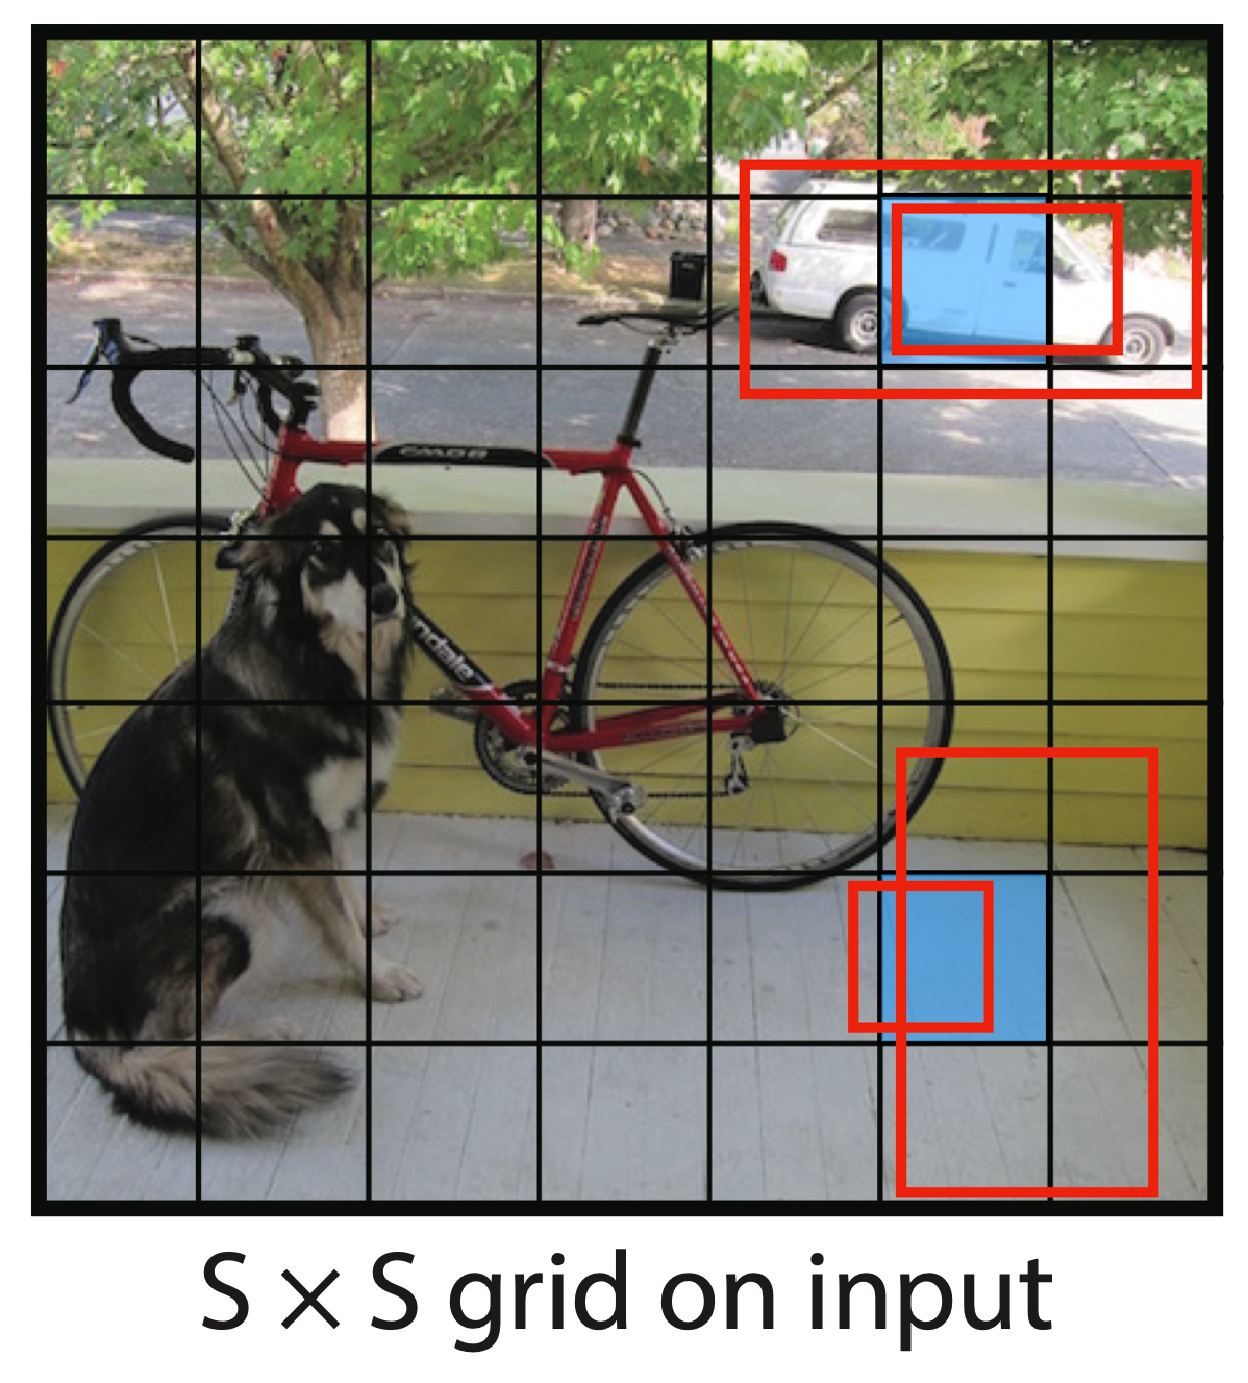
\includegraphics[height=0.4\textheight]{../graphics/YOLO_2.pdf}
   \caption{YOLO: the image is partitioned by an $S \times S$ grid.}
\end{figure}
\begin{itemize}
   \item First, the image is divided into a $S \times S$ grid of cells. 
   \item For each of these cells, we will then predict:
   \begin{itemize}
      \item Location and size of $B$ different boxes. 
      \item A confidence score that the box contains an object. 
      \item The class of the object in each of the $B$ boxes. 
   \end{itemize}
\end{itemize}
\end{frame}

% \begin{frame}{YOLO: confidence score of a predicted box}
% % \begin{figure}[htb]
% %    \centering
% %    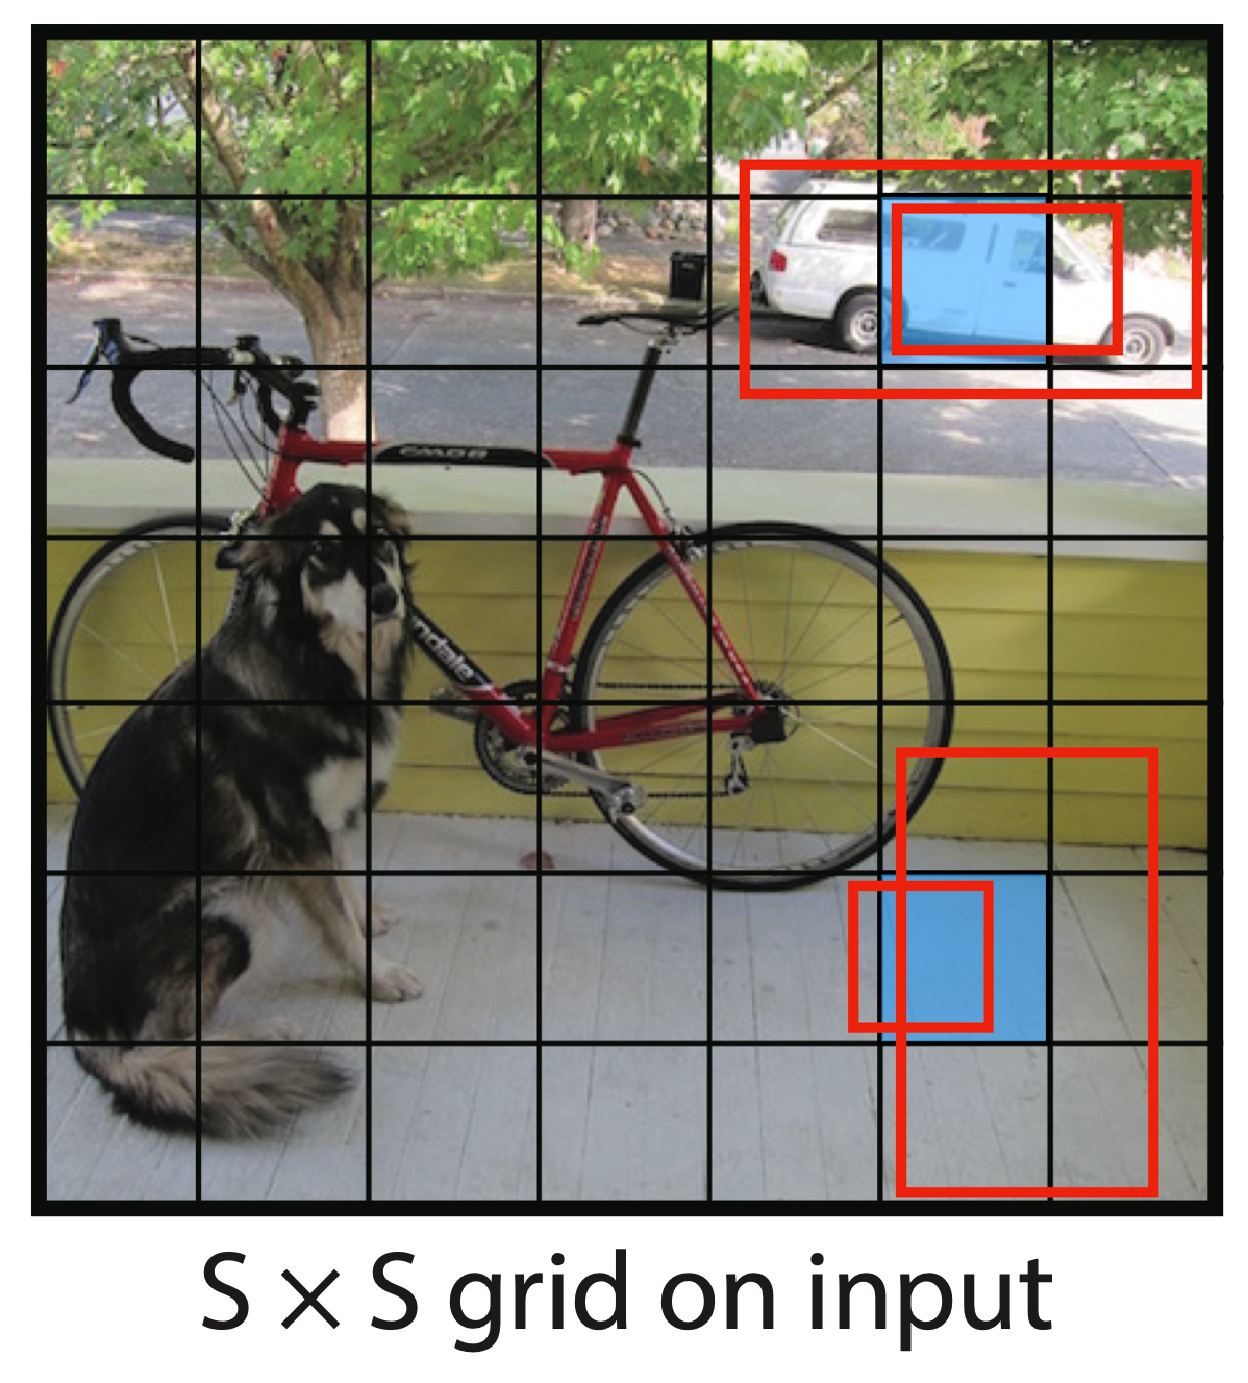
\includegraphics[height=0.4\textheight]{../graphics/YOLO_2.pdf}
% %    \caption{YOLO: the image is partitioned by an $S \times S$ grid.}
% % \end{figure}
% \begin{itemize}
%    \item The confidence score of a predicted bounding box $\hat{B}_i$ is defined as:
%    \begin{equation}
%       Conf_i = P(Obj) IOU(\hat{B}_i, B_i)
%    \end{equation}
%    \item The confidence score is thus close to 0 if there is no object associated in the bounding box. 
%    \item Otherwise the confidence score corresponds to the intersection over union ($IOU$). 
%    \item The confidence score thus represents both the probability of an object and the localization quality of the predicted box.  
% \end{itemize}
% \end{frame}


\begin{frame}{YOLO: each cell predicts boxes and confidences}
% \begin{figure}[htb]
%    \centering
%    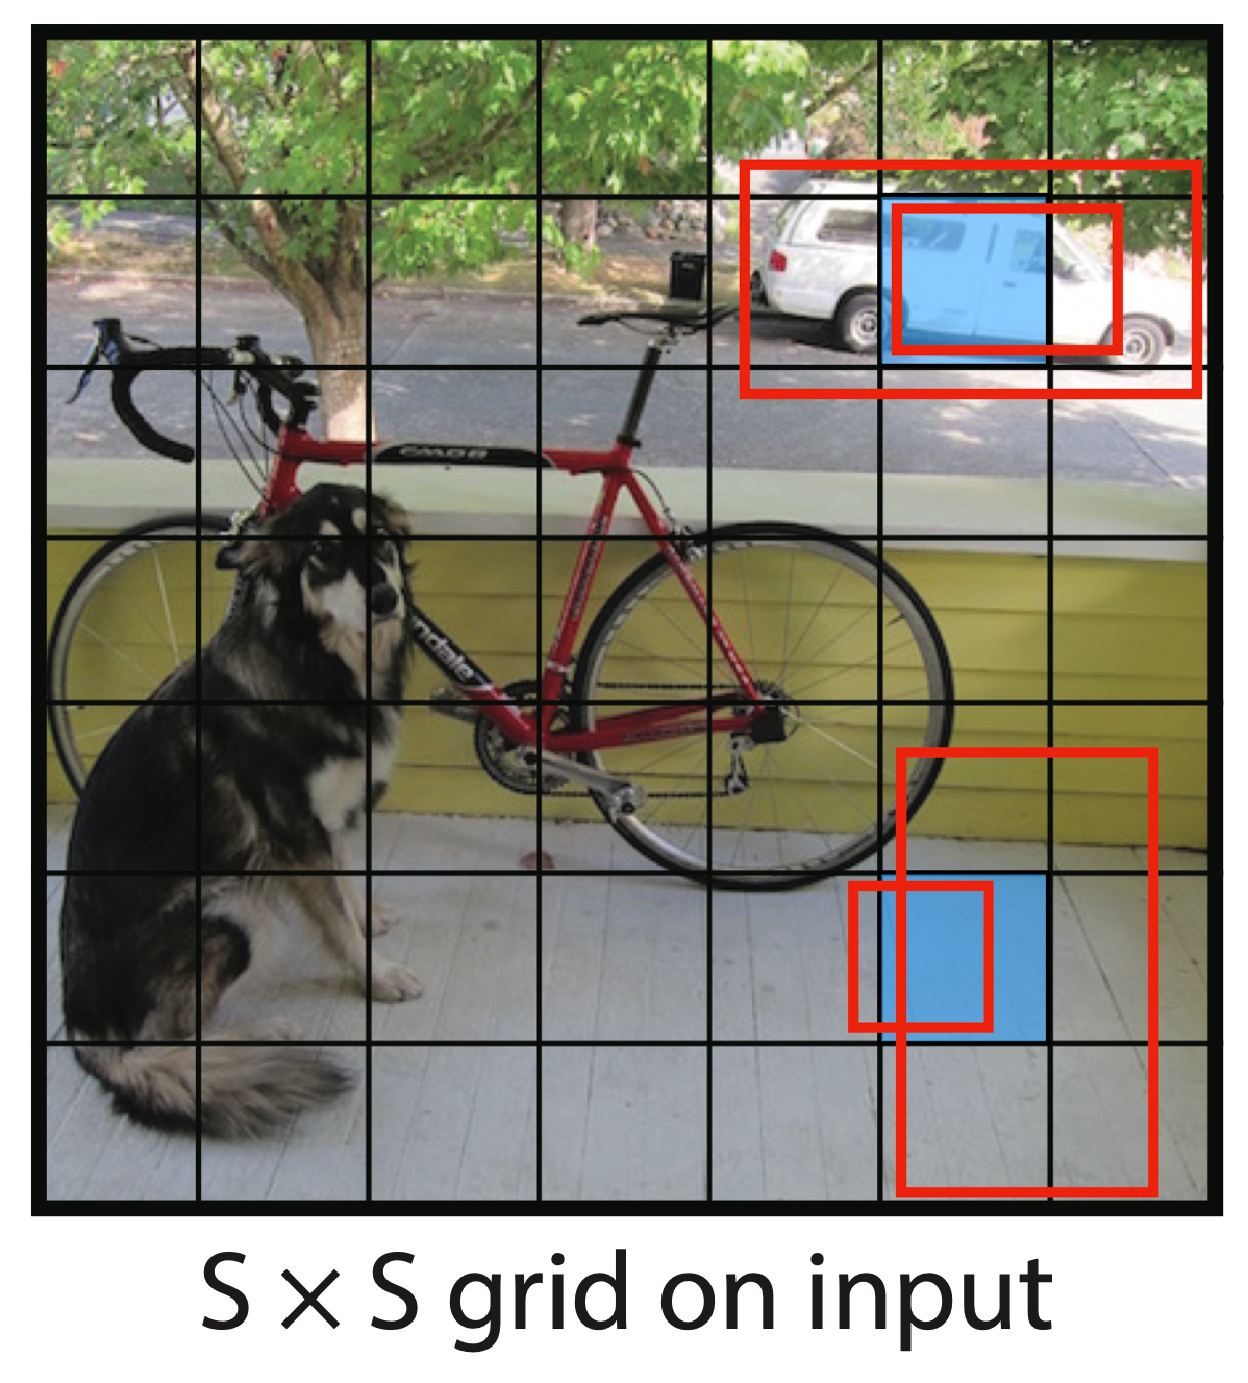
\includegraphics[height=0.4\textheight]{../graphics/YOLO_2.pdf}
%    \caption{YOLO: the image is partitioned by an $S \times S$ grid.}
% \end{figure}
\begin{itemize}
   \item If the center of an object falls into one cell, that cell is responsible for the prediction of the object. 
   \item Geometry and position of the bounding box: 
   \begin{itemize}
      \item Center $(x, y)$ with respect to the origin of the cell.
      \item The relative width and height: $w$, $h$ (normalized by image width and height). 
   \end{itemize}
   \item The confidence score of a predicted bounding box $\hat{B}_i$ is defined as:
   \begin{equation}\nonumber
      Conf_i = P(Obj) IOU(\hat{B}_i, B_i)
   \end{equation}
   where $B_i$ is the ground truth bounding box. 
   \item At test time the confidence values $Conf_i$ are predicted (together with the bounding box geometry). 
\end{itemize}
\end{frame}

\begin{frame}{YOLO: prediction of the class}
\begin{figure}[htb]
   \centering
   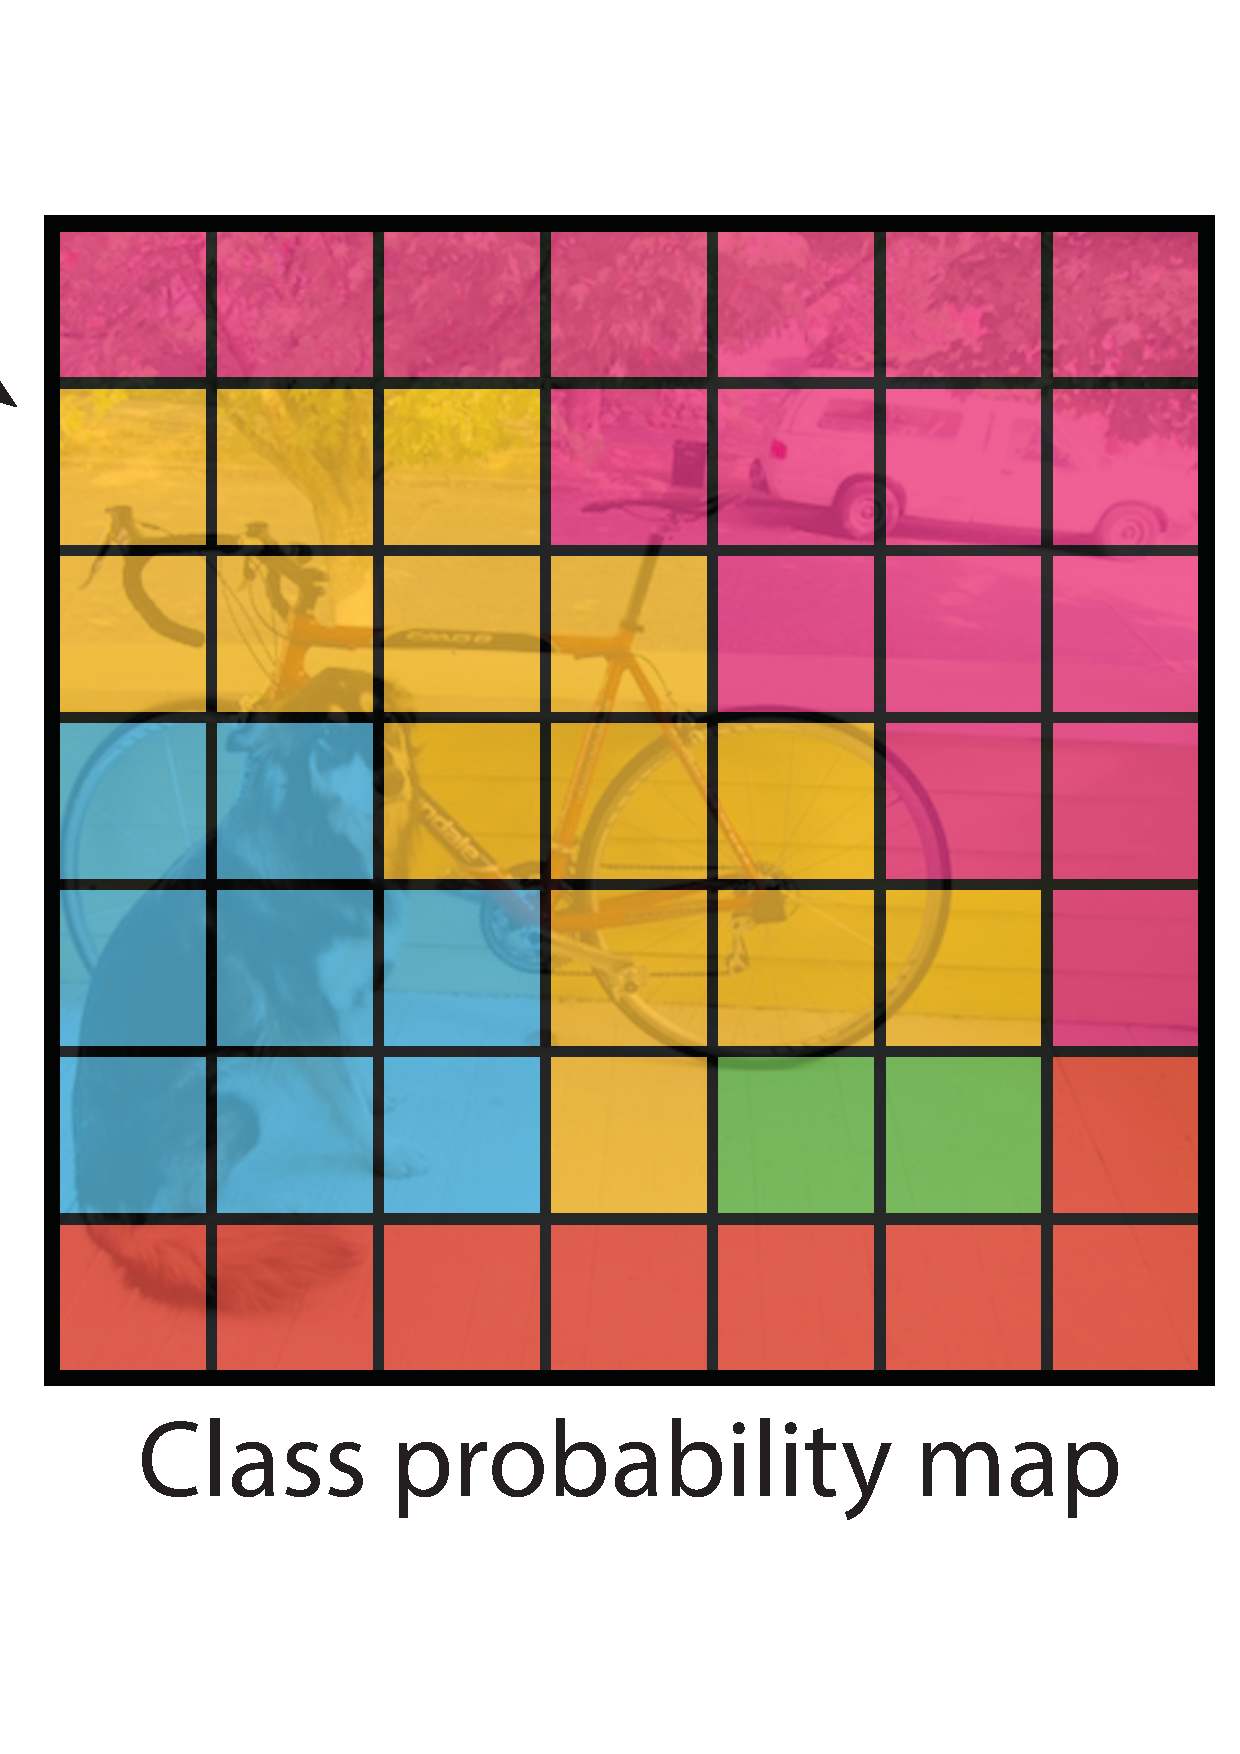
\includegraphics[height=0.4\textheight]{../graphics/YOLO_ClassProbabilityMap.pdf}
   \caption{Class map prediction}
\end{figure}
\begin{itemize}
\item Each cell of the partition predicts also $K$ class probabilities, conditioned on the presence of an object $P(C_i|obj)$. 
\item During prediction, this class probability is multiplied with the confidence score:  
\begin{equation}\nonumber
P(C_k|obj) Conf = P(C_k | obj) P(obj) IOU(\hat{B}, B) = P(C_k) IOU(\hat{B}, B)
\end{equation}
This provides class-specific confidence scores for each of the predicted boxes. 
\end{itemize}
\end{frame}

\begin{frame}{YOLO: Output}
\begin{figure}[htb]
   \centering
   \includegraphics[height=0.4\textheight]{../graphics/YOLO_Output.pdf}
   \caption{Output layer of YOLO for 5 classes}
\end{figure}
If we assume that our initial grid was $7 \times 7$, we predict two boxes per cell and that we have 20 classes, we obtain as output layer a tensor of dimension: 
\begin{equation}\nonumber
(7 \times 7) \times (2 \times 5 + 20) = 1470
\end{equation}
This is the number of output variables we would predict. 
\end{frame}


\begin{frame}{YOLO: Examples}
\begin{figure}[htb]
   \centering
   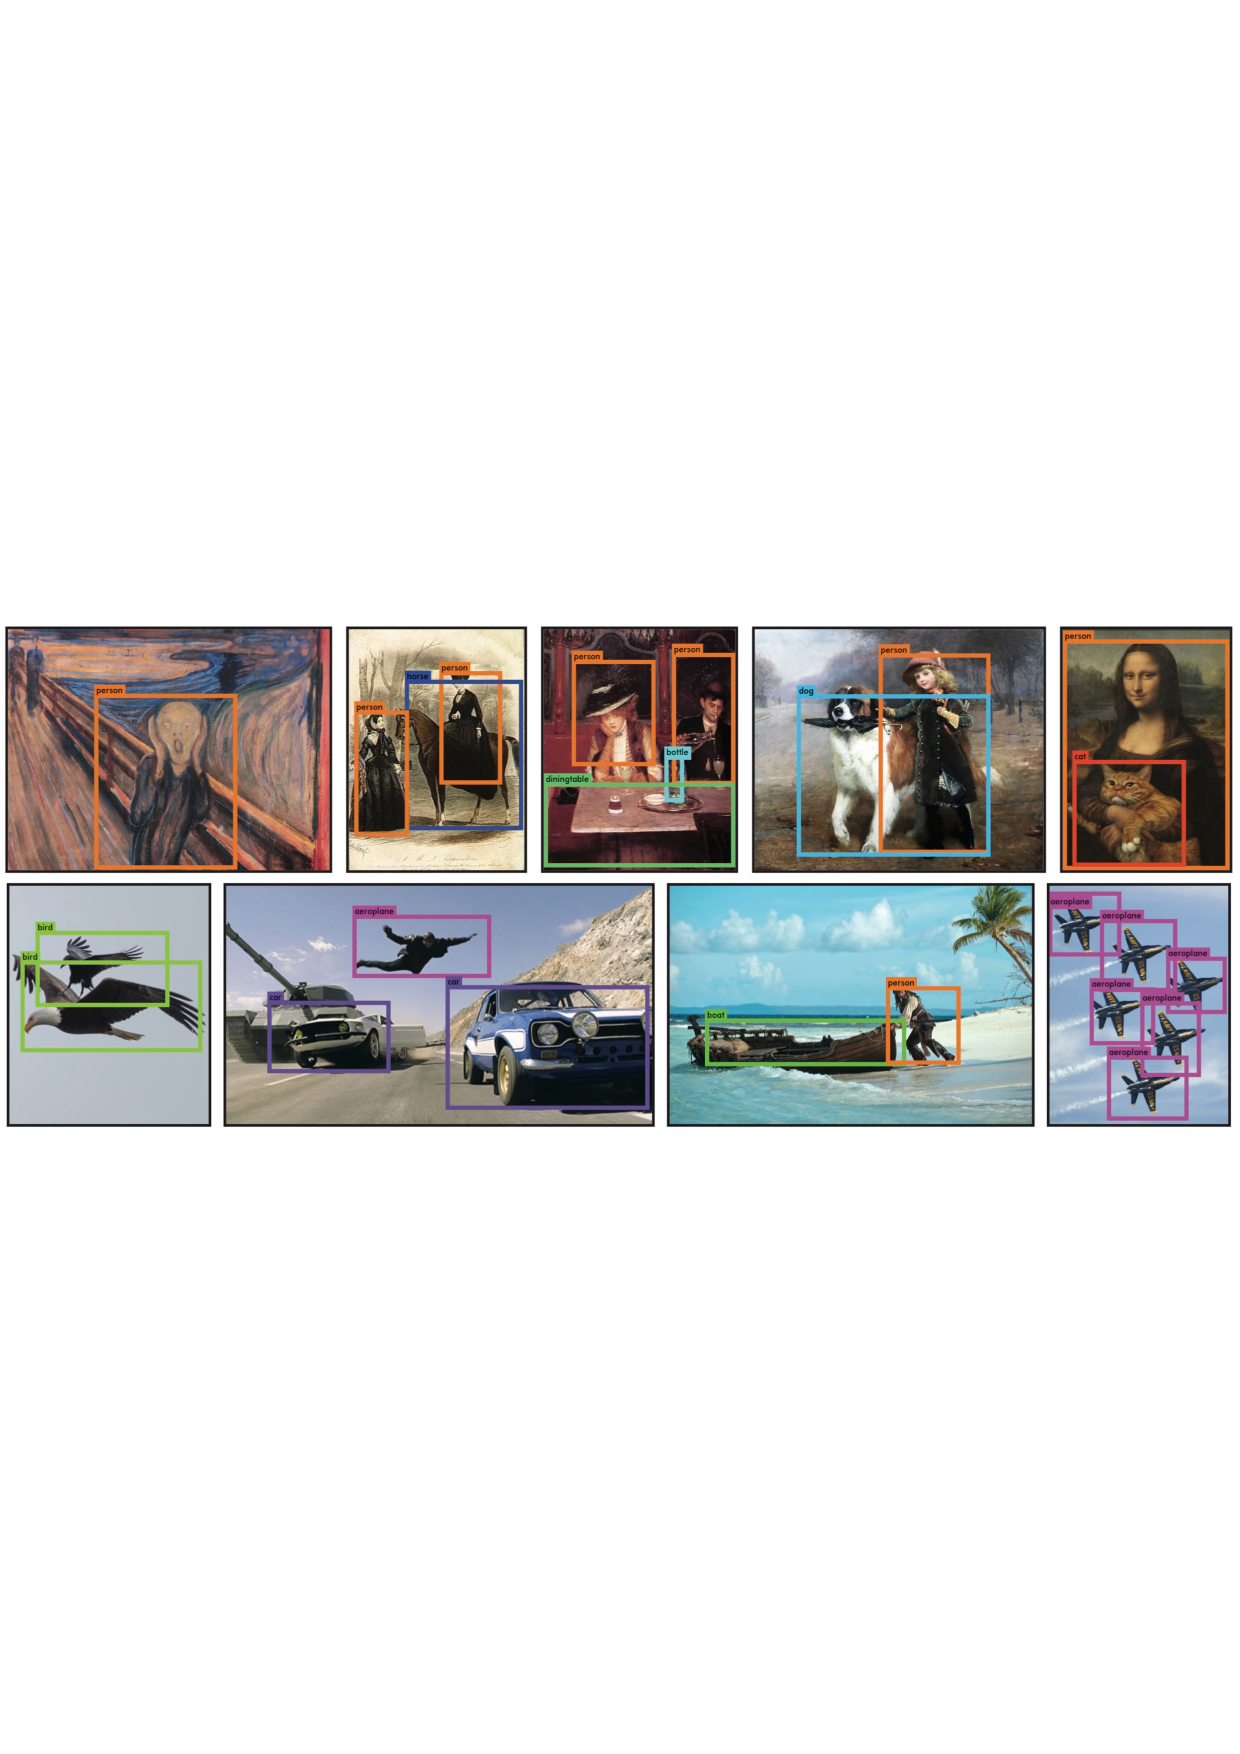
\includegraphics[width=\textwidth]{../graphics/YOLO_ex.pdf}
   \caption{Examples for YOLO detections}
\end{figure}
The method is extremely fast. Localization is less precise than for Faster R-CNN. 
\end{frame}


% \begin{frame}{Multiple Instance Segmentation}

% \end{frame}

\section{Conclusion}

\begin{frame}{Conclusion}
\begin{itemize}
\item Object detection is a major challenge in Computer Vision with applications in biomedical image analysis, autonomous driving, industrial applications, etc.
\item CNNs outperform most traditional methods by a large margin. 
\item Today, object detection is among the most stunning applications of Computer Vision. 
\item There are hundreds of methods, but the most important advances were achieved by R-CNN, Fast R-CNN, Faster R-CNN and YOLO. 
\item They can be combined with segmentation (Mask R-CNN). 
\end{itemize}
\end{frame}

%The conv-layers are determined by first training the RPN (ImageNet initialization), then we train Fast R-CNN for the proposed regions (again with ImageNet initialization). The shared layers are then frozen.

%\item RPN and classification network thus share the conv-layers. They are specialized later. 

%%%%%%%%%%%%%%%%%%%%%%%%%%%%%%%%%%%%%%%%%%%%%%%%%%%%%%%%%%%%%%%%%%%%%%%%%
%%%%%%%%%%%%%%%%%%%%%%%%%%%%%%%%%%%%%%%%%%%%%%%%%%%%%%%%%%%%%%%%%%%%%%%%%
\section{References}
\begin{frame}[allowframebreaks]
	\frametitle{References}
	\bibliography{object_detection.bib}
\end{frame}


\end{document}
